%!TeX TS-program = pdflatex
%!TeX encoding = UTF-8 Unicode
%!TeX spellcheck = en-US
%!BIB TS-program = bibtex
% -*- coding: UTF-8; -*-
% vim: set fenc=utf-8
%: METADATA
%: %%%%%%%%%%%%%%%%%%%%%%%%%%%%%%%%%%%%%%%%%%%%%%%%%%%%%%%%%%%%%%%%%%%%
\newcommand{\AuthorA}{Chlo\'e Pasturel}
\newcommand{\AuthorB}{Anna Montagnini}%
\newcommand{\AuthorC}{Laurent U.~Perrinet}%
\newcommand{\Address}{Institut de Neurosciences de la Timone, CNRS / Aix-Marseille Universit\'e - Marseille, France}%
\newcommand{\Website}{http://invibe.net/LaurentPerrinet}%
\newcommand{\Email}{Laurent.Perrinet@univ-amu.fr}%
\newcommand{\Title}{
%Principles and psychophysics of Active Inference in anticipating a dynamic probabilistic bias
Humans adapt to the volatility of visual motion properties, and know about it
%Anticipating a volatile probabilistic bias in visual motion direction
%Humans adapt to the volatility of visual motion properties :  eye movements and explicit guesses
}
\newcommand{\Acknowledgments}{PACE-ITN - code and material @ \url{\Website/Publications/Pasturel_etal2018}. TODO: RIck + Karl + JB + Laurent Madelain }
\newcommand{\Abstract}{
The brain has to constantly adapt to changes in the environment, for instance when a contextual probabilistic variable switched its state.
For an agent interacting with such an environment, it is important to respond to such switches with the shortest delay.
However, this operation has in general to be done with noisy sensory inputs and solely based on the information available at the present time.
Here, we tested the ability of humans observers to accurately anticipate, with their eye movements, a target's motion direction throughout random sequences of rightward/leftward motion alternations, with random-length contextual blocks of different biases in direction probability. 
Experimental results were compared to those of a probabilistic agent optimized with respect to this switching model.
We found a good fit of the behaviorally observed anticipatory response compared with other models such as the leaky-integrator model.
Moreover, we could also fit the level of confidence given by human observers with that provided by the model. 
Such results provide evidence that human observers may efficiently represent an anticipatory belief along with its precision and they support a novel approach to more generically test human cognitive abilities in uncertain and dynamic environments.
}
%%%%%%%%%%%%%%%%%%%%%%%%%%%%%%%%%%%%%%%%%%
\documentclass[profile,final,english, draft]{article}%
\usepackage{babel}
% MATHS (AMS)
\usepackage{amsmath}
\usepackage{amsfonts} 
\usepackage{amssymb}
\usepackage{amsthm}
\newcommand{\KL}[2]{\text{KL}( #1 | #2 )}
%% parenthesis
\newcommand{\pa}[1]{\left( #1 \right)}
\newcommand{\bpa}[1]{\big( #1 \big)}
\newcommand{\choice}[1]{ %
	\left\{ %
		\begin{array}{l} #1 \end{array} %
	\right. }
% ensembles
\newcommand{\ens}[1]{ \{ #1 \} }
\newcommand{\enscond}[2]{ \left\{ #1 \;;\; #2 \right\} }
% egal par définition
\newcommand{\eqdef}{\ensuremath{\stackrel{\mbox{\upshape\tiny def.}}{=}}}
\newcommand{\eqset}{\ensuremath{\stackrel{\mbox{\upshape\tiny set}}{=}}}
\newcommand{\eq}[1]{\begin{equation*}#1\end{equation*}}
\newcommand{\eql}[1]{\begin{equation}#1\end{equation}}

\DeclareMathOperator{\argmin}{argmin}
\DeclareMathOperator{\argmax}{argmax}
\newcommand{\uargmin}[1]{\underset{#1}{\argmin}\;}
\newcommand{\uargmax}[1]{\underset{#1}{\argmax}\;}
\newcommand{\umin}[1]{\underset{#1}{\min}\;}
\newcommand{\umax}[1]{\underset{#1}{\max}\;}
\newcommand{\usup}[1]{\underset{#1}{\sup}\;}
% for units
\usepackage{siunitx}%
\newcommand{\ms}{\si{\milli\second}}%

%% Symboles arrondis
\newcommand{\Aa}{\mathcal{A}}
\newcommand{\Bb}{\mathcal{B}}
\newcommand{\Cc}{\mathcal{C}}
\newcommand{\Dd}{\mathcal{D}}
\newcommand{\Ee}{\mathcal{E}}
\newcommand{\Ff}{\mathcal{F}}
\newcommand{\Gg}{\mathcal{G}}
\newcommand{\Hh}{\mathcal{H}}
\newcommand{\Ii}{\mathcal{I}}
\newcommand{\Jj}{\mathcal{J}}
\newcommand{\Kk}{\mathcal{K}}
\newcommand{\Ll}{\mathcal{L}}
\newcommand{\Mm}{\mathcal{M}}
\newcommand{\Nn}{\mathcal{N}}
\newcommand{\Oo}{\mathcal{O}}
\newcommand{\Pp}{\mathcal{P}}
\newcommand{\Qq}{\mathcal{Q}}
\newcommand{\Rr}{\mathcal{R}}
\newcommand{\Ss}{\mathcal{S}}
\newcommand{\Tt}{\mathcal{T}}
\newcommand{\Uu}{\mathcal{U}}
\newcommand{\Vv}{\mathcal{V}}
\newcommand{\Ww}{\mathcal{W}}
\newcommand{\Xx}{\mathcal{X}}
\newcommand{\Yy}{\mathcal{Y}}
\newcommand{\Zz}{\mathcal{Z}}
%% ========  polices de caracteres =============
\usepackage[T1]{fontenc}% 
\usepackage{lmodern}%
\usepackage{t1enc}
\usepackage{ragged2e}
%============ graphics ===================
\usepackage[pdftex]{graphicx}% 
\DeclareGraphicsExtensions{.pdf,.png,.jpg}%
\graphicspath{{./figures/}}%
%\usepackage[numbers,comma,sort&compress,round]{natbib} %
\usepackage[%style=nature,
maxcitenames=2,
maxnames = 2,
firstinits=true,
uniquename=init,
sorting=none,
url=false,
isbn=false,
eprint=false,
texencoding=latin1,
bibencoding=utf8,
autocite=superscript,
backend=bibtex,
%articletitle=false
]{biblatex}%
\addbibresource{Pasturel_etal2018.bib}%
\newcommand{\citep}[1]{(\cite{#1})}
%\newcommand{\citet}[1]{(\textcite{#1})}
%%%%%%%%%%%%%%%%%%%%%%%%%%%%%%
%% OPTIONAL MACRO FILES
%\usepackage{tikz,tkz-euclide} \usetkzobj{all} % loading all objects
%\usetikzlibrary{positioning} \usetikzlibrary{calc}
%\usepackage{sfmath}
%============ hyperref ===================
\usepackage[unicode,linkcolor=red,citecolor=red,filecolor=black,urlcolor=red,pdfborder={0 0 0}]{hyperref}%
\hypersetup{%
pdftitle={\Title},%
pdfauthor={\AuthorA},%< \Email > \Address},%
}%
\usepackage{color}%
%%%%%%%%%%%%%%%%%%%%%%%%%%%%%%%%%%%
\title{\Title}%
\author{\AuthorA, 
\AuthorB,  
\AuthorC\thanks{\Address} }

%%%%%%%%%%%% Her begynner selve dokumentet %%%%%%%%%%%%%%%
\begin{document}%
\maketitle%
%%%%%%%%%%%%%%%%%%%%%%%%%%%%%%%%%%%%%%%%%%%%%%%%%%%%%%%%%%%%%%%%
%: Abstract
\begin{abstract}
\Abstract
\end{abstract}
%: %%%%%%%%%%%%%%%%%%%%%%%%%%%%%%%%%%%%%%%%%%%%%%%%%%%%%%%%%%%%%%%
\section{Motivation}
%%%%%%%%%%%%%%%%%%%%%%%%%%%%%%%%%%%%%%%%%%%%%%%%%%%%%%%%%%%%%%%%
%%%%%%%%%%%%%%%%%%%%%%%%%%%%%%%%%%%%%%%%%%%%%%%%%%%%%%%%%%%%%%%%
%%%%%%%%%%%%%%%%%%%%%%%%%%%%%%%%%%%%%%%%%%%%%%%%%%%%%%%%%%%%%%%%
\subsection{Volatility of sensory contingencies and the adaptation of cognitive systems}
% --------------------------------------------------------------------------------------
%: general volatility
 We live in a fundamentally volatile world - Think for instance to 
 * the evolution  of prices on the stock market: Any Socio-economic contextual index may make the price evolve up or down, slowly or more Rapidly    
 * ecological change 
 * the side (left or right of the field) in which the ball is on a soccer field

 
 essential to infer near future state in a dynamic environment - or at least to get an idea for the future context / link to reinforcement learning
define our time scale: adaptive response (several minutes) - stimulus history and psychophysics
 
% 
%Perceptual learning mainly produces improvements in discrimination with long-term training on a perceptual judgement~\citep{Lu2009}. On the other hand, adaptation is typically characterized as an imminent loss in sensitivity to a stimulus's exposure. Recent examples of positive biases in perceptual discrimination are numerous and shows that the visual system tends to favor stimulus' temporal and spatial stability~\citep{Burr2014, Fischer2014, Liberman2014}. For instance, facilitatory effects such as priming enhance the stimulus identification of repeated motion~\citep{Verstraten1994, Tiest2009}. Additionally, those integration mechanisms tend to share the same neural substrates~\citep{Campana2002, Campana2006, Campana2013}. The ability to detect sequential regularities then appears as a fundamental ability for the adaptive behavior of species. On various experiments, learning of local sequence have been observed even on randomized events or with restrained contingencies~\citep{Squires1976, Strauss2015}. Namely in two-alternative forced-choices studies that have revealed "sequential effects", i.e. fluctuations in performance induced by the local regularities in the sequence of events. A same response presented several times could indeed lead to faster and more accurate responses and, on the other hand, lead to impairment in the behavior when a presented stimulus was going against the expected belief~\citep{Hyman1953, Yu2009}. Other studies also report that when participants are asked to to produce random sequences and to rate the randomness of those, they show an underestimation of the likelihood of alternations~\citep{Sun2015, Kareev1995}. One remaining question though, is to select a model approach to those phenomenon and how sequential effects are integrated. Nowadays, the Bayesian inference is an effective approach to deal with this question.
%
 
 
%: Past history of sensory event integration
Stimulus history of events influences how current stimuli are perceived and acted upon, mostly by using adaptability features to environment contingencies. One of the adaptation process' main purpose is to reduce the sensitivity to stimuli recently presented and thus re-calibrate perceptual experience~\citep{Clifford2007, Webster2011, Kohn2007}. This process is highly dynamic especially in complex environments where new contingencies can arise at every moment. In the case of visual motions, the process of visual adaptation in mostly defined by repeated exposures of stimuli and after-effects related to those statistical regularities~\citep{Thompson2009}. Thus, it is interesting to note that a large variety of dynamic of an environment has a direct dependency with previous experience. The coding of a visual event then, relies in the integration of the recent past but also to catch sudden changes in the spatial context that would go against an~\textit{a priori} belief. We can illustrate this statement with several examples, such as 1/ Motion Aftereffect: Prolonged exposure to a stimulus moving in one direction result in a motion aftereffect and the presentation of a stationary stimulus is perceived to move in the opposite direction of the adapting stimulus~\citep{Anstis1998, Mather2011}. The motion aftereffect usually builds up over time~\citep{Hershenson1993}, sometimes after relatively short exposures~\citep{Kanai2005, Pavan2010} and can last for period of ten seconds~\citep{Anstis1998}. Interestingly, it can be integrated in memory over relatively long-period without further stimulations~\citep{Verstraten1994, Wiesenfelder1992}; 2/ Priming: In the case of priming, repeated stimulations creates a facilitation in perception~\citep{Kristjnsson2010WherePM, Maljkovic1994, Tulving1990}. Indeed, after exposure to a similar stimulus, priming leads to faster responses in perceptual detection or identification of probes. It also occurs specifically for visual motion stimuli~\citep{Anstis1987, Campana2002, Pinkus1997}. Interestingly, observation of priming effects have been observed for anticipatory smooth eye movements (aSPEM). 
% TODO add saccadic adaptation

%: role of predictive processing in shaping this adaptive response
See Matthys and Meyniel
Chopin and Mamassian
Mamassian and the use of visual confidence  (see Ann rev of Vision 2016)

Necessity of using a generative model
%A key principle in the Bayesian inference approach is the hypothesis that information is processed by the brain by computing probabilities~\citep{Deneve1999, Diaconescu2014}. Then this probabilistic computations follows a Bayes's rule and infer the hidden regularities of received inputs~\citep{Deneve1999, Hoyer2003, Ma2014}. Afterward, the brain combines the likelihood of observations given putative regularities and the prior likelihood of these regularities~\citep{Janes2014}. A final principle is the predictive and iterative nature of bayesian models. Once the hidden regularities of the inputs are referred, they are used by the brain to anticipate the likelihood of future observations. Thus, the comparisons between expectations and actual data produces a constant update the estimates of the model under a mechanism that is labelled as the~\textit{active inference}~\citep{Friston2003, Friston2010}. In a study,~\citet{Meyniel2016} simulated a model over five different set of datas previously published~\citep{Squires1976, Huettel2002, Kolossa2013, Cho2002, Falk1997}. Their main conclusion was that only a learning of local transition probabilities was compatible with the large repertoire of experimental effects reported here and could be summarized in six assumptions:
%
%\begin{enumerate}
%\item Expectations derived from such a learning show effects of both the frequencies of items and their alternations because these statistics are specific aspects of transition probabilities,
%\item These effects emerge both globally and locally in the learning process because the inference is non-stationary,
%\item This non-stationarity also entails that local effects emerge even in purely random sequences,
%\item It depends on the exact order of observations within the local history,
%\item Since the space of transition probabilities is more general that the frequencies of items and their alternations, the local transition probability model makes a non-trivial prediction prediction, unaccounted for by simpler statistics: expectations build up more strongly from repetitions than from alternations,
%\item Signatures of expectations and their violation in human behavior observed on reaction times measures and brain signals (electrophysiology and fMRI) conformed both qualitatively and quantitatively the upper predictions.
%\end{enumerate}
%
%Work of~\citet{Meyniel2016} concluded that transitions probabilities constitute a core building block of sequence knowledge in the brain, which then applies to a variety of sensory modalities and experimental situations. It also suggests that, during sequences of learning, the system considers a space of hypothesis that is more general than previously though. Sequential effects in binary sequences are better explained by a learning of transition probabilities than of the absolute item frequencies or the frequencies of their alternations. A main point was that all of those models have the same numbers of free parameters, so that the local transition probability model is more general without being more complex or less constrained. The critical difference lies in the content of what is learned (item frequencies versus transition probabilities). More generally, Bayesian models may consider a vast hypothesis space~\citep{Kemp2008} and then attempt to capture human behavior. To do so, a very few or even zero adjustable parameters may be necessary.
%


% --------------------------------------------------------------------------------------
\subsection{Anticipatory SPEM (aSPEM)}
% --------------------------------------------------------------------------------------
%: adaptation to volatility is seen as an anticipation in SPEM - principle and function (talk about santos & kowler and others)
Humans are able to accurately track a moving object with a combination of saccades and smooth eye movements. These movements allow us to align and stabilize the object on the fovea, thus enabling high-resolution visual detection. When predictive information is available about target motion, anticipatory smooth pursuit eye movements (aSPEM) are efficiently generated before target appearance, which reduce the typical sensorimotor delay between target motion onset and foveation. It is generally assumed that the role of anticipatory eye movements is to limit the behavioral impairment due to eye-to-target position and velocity mismatch.

%: how we do it
%Repeated presentation of stimulus can lead the oculomotor system to initiate aSPEM ahead of the stimulus appearance~\citep{Westheimer1954, KOWLER1979619, KOWLER1979633}. It has been observed that aSPEM increase in velocity when the target repeatedly moves in the same direction~\citep{Kowler1984, Kowler1989, Heinen2005}. Thus,~\citet{Maus2015} have recently shown that both perceptual adaptation and priming of aSPEM could occur simultaneously. They found a robust repulsive adaptation effect with perceptual judgements being biased faster after seeing stimuli that were slower and~\textit{vice-versa}. This study clearly shows the integration of past event and their usefulness in actual eliciting of movements. Indeed, both priming and adaptation can hypothetically share a common internal representation of stimulus speed that has been build upon the mean velocity of last encountered speeds. Then the comparison of the internal representation of speed with the current stimulus velocity could explain repulsive aftereffects and at the same time, be used to elicit aSPEM of appropriate velocity for next stimulus occurrences.~\citet{Maus2015} main conclusion was that perceptual adaptation and oculomotor priming both have a weight in building an~\textit{a priori} knowledge that will be used to generate aSPEM. Still, they integrated past history over different times scales (see fig~\ref{fig:Maus2015.png}) with the priming effects being maximized for short stimulus histories (around 2 trials) and adaptation for longer stimulus history, around 15 trials. Such history length can still be considered short history namely in the case of several hundreds blocks of trials like we did in our first study.

%: in summary we get a linear relationship
By manipulating the probability for target motion direction we were able to bias the direction and mean velocity of aSPEM, as measured during a fixed duration gap before target ramp-motion onset. This suggests that probabilistic information may be used to inform the internal representation of motion prediction for the initiation of anticipatory movements~\parencite{Montagnini2010}. However, such estimate may become particularly challenging in a dynamic context, where the probabilistic contingencies vary in time in an unpredictable way. In addition, whether and how the information processing underlying the buildup of aSPEM is linked to an explicit estimate of probabilities is unknown. We developed a new paired-task paradigm in order to address these two questions. In a first session, participants observe a target moving horizontally with constant speed from the center either to the right or left across trials. The probability of either motion direction changes randomly in time. Participants are asked to estimate "how much they are confident that the target will move to the right or left in the next trial" and to adjust the cursor's position on the screen accordingly. In a second session the participants eye movements are recorded during the observation of the same sequence of random-direction trials.


% --------------------------------------------------------------------------------------
\subsection{Target of this paper}
% --------------------------------------------------------------------------------------
%: limits of the previous method
Fixed block. does this generalize to arbitrtary sequences? What is the dynamic of this adaptation?
Models which only mimick the behaviour (Souto for saccadic adaptation) without explaining it but see Meyniel
The HGF of Matthys is 1/ great 2/ way too complicated for the type of behaviours we want to explain

%: design of the binary switching generative model
%\subsection{Generative model: the switching model}
Hierarchical model of 3 layers: "hardest model" all information is controlled - no artefact possible by using the gernrative model

In order to answer these questions, we have set up an experiment comprising $3$ blocks of $200$ trials, see Figure~\ref{fig:results_raw}-A\footnote{Each block is divided in 4 sub-blocks of $50$ trials as denoted by vertical black bars}. For each trial, a target makes either to the left or to the right, this direction being drawn from a Bernoulli process. The probability of this process varied in a piecewise-constant (that is, a step function varying between~$0$ and~$1$), similarly to~\textcite{Meyniel13}. The occurrence of these switches is itself drawn from a Bernoulli process of probability $p_{switch}=1/40$.

\eql{\choice{
x_0^t \eqdef o_t \propto \Bb(p^t) \\
x_1^t \eqdef p_t = p_{t-1} \quad \text{if} \quad s_t=0 \quad \text{and else} \quad p_t \propto \Jj \\
x_2^t \eqdef s_t \propto \Bb(\lambda) 
}}

where $\Jj = BB(\frac 1 2 , \frac 1 2 )$ is Jeffrey's prior (TODO: put in appendix). There is always a switch at t=zero.
allows to generate blocks

% * This was shown to happen in the more  experimental setting While recording smooth pursuit eye movements : Anna Montagnini has previously shown that if you use a probabilistic bias in the direction of the movement of the target, the the eye will (uncousciously) anticipate in the direction of this bias.
%
% * this protocol used a random length fixation period then a pause of fixed duration, and then a traget moving at 15 deg / s
%
% * the value p gives the probability of going to the right : at .5 it is unbisaed, and at .75 for instance it goes 75% to the right and 25% to the left
% 



Throughout the first experimental condition we investigated the integration of environmental statistical regularities in a smooth tracking task with a family of direction-biases for the target motion. What we found was a global and robust effect of direction-bias on anticipatory smooth pursuit. These results are coherent with previous oculomotor findings by our and also other groups (Montagnini et al. 2010; Santos \& Kowler 2017). Typically, aSPEM is observed after a temporal cue and ahead of target motion onset (Kowler and Steinman, 1979a,b, 1984). Some now classical experiments have demonstrated the existence of prediction-based smooth pursuit during the transient disappearance of a moving target (Badler, 2006; Becker \& Fuchs, 1985). Overall, it is now clear that smooth pursuit behavior can be modulated even in the absence of online sensory stimulation. aSPEM were here the core of our research because we wanted to study the trial-by-trial evolution of expectancy-based oculomotor behavior, as well as how sensorimotor expectancy interacts with reward contingencies in shaping oculomotor behavior without direct sensory feedback. In a previous study, (Souto, Montagnini \& Masson, 2008b; Montagnini et al., 2010) we have analyzed how forthcoming motion properties, such as target speed or direction, can be predicted and anticipated with coherent orienting eye movements. We found a graded effect of both the speed and the direction-bias, with mean anticipatory eye velocity linearly related to the probability of motion's speed or direction. Here, we replicated part of those results using a limited number of direction probability bias and strengthened them by generalizing them on seventeen participants. These results imply that the probability bias over a target's direction is one additional factor beyond other physical and cognitive cues (Kowler et al, 2014; Santos \& Kowler 2017) that modulate the common predictive framework driving anticipatory behavior to optimize a rapid and precise foveation of the target on its most expected future path. 
%Montagnini A, Souto D, and Masson GS (2010) <a href="http://jov.arvojournals.org/article.aspx?articleid=2138664">J Vis (VSS Abstracts) 10(7):554</a>,<BR> Montagnini A, Perrinet L, and Masson GS (2015) <a href="https://arxiv.org/abs/1611.07831">BICV book chapter</a>


%-------------------------------------------------------------%
%: FIGURE 1 fig:intro
\begin{figure}%[b!]
%\begin{center}
%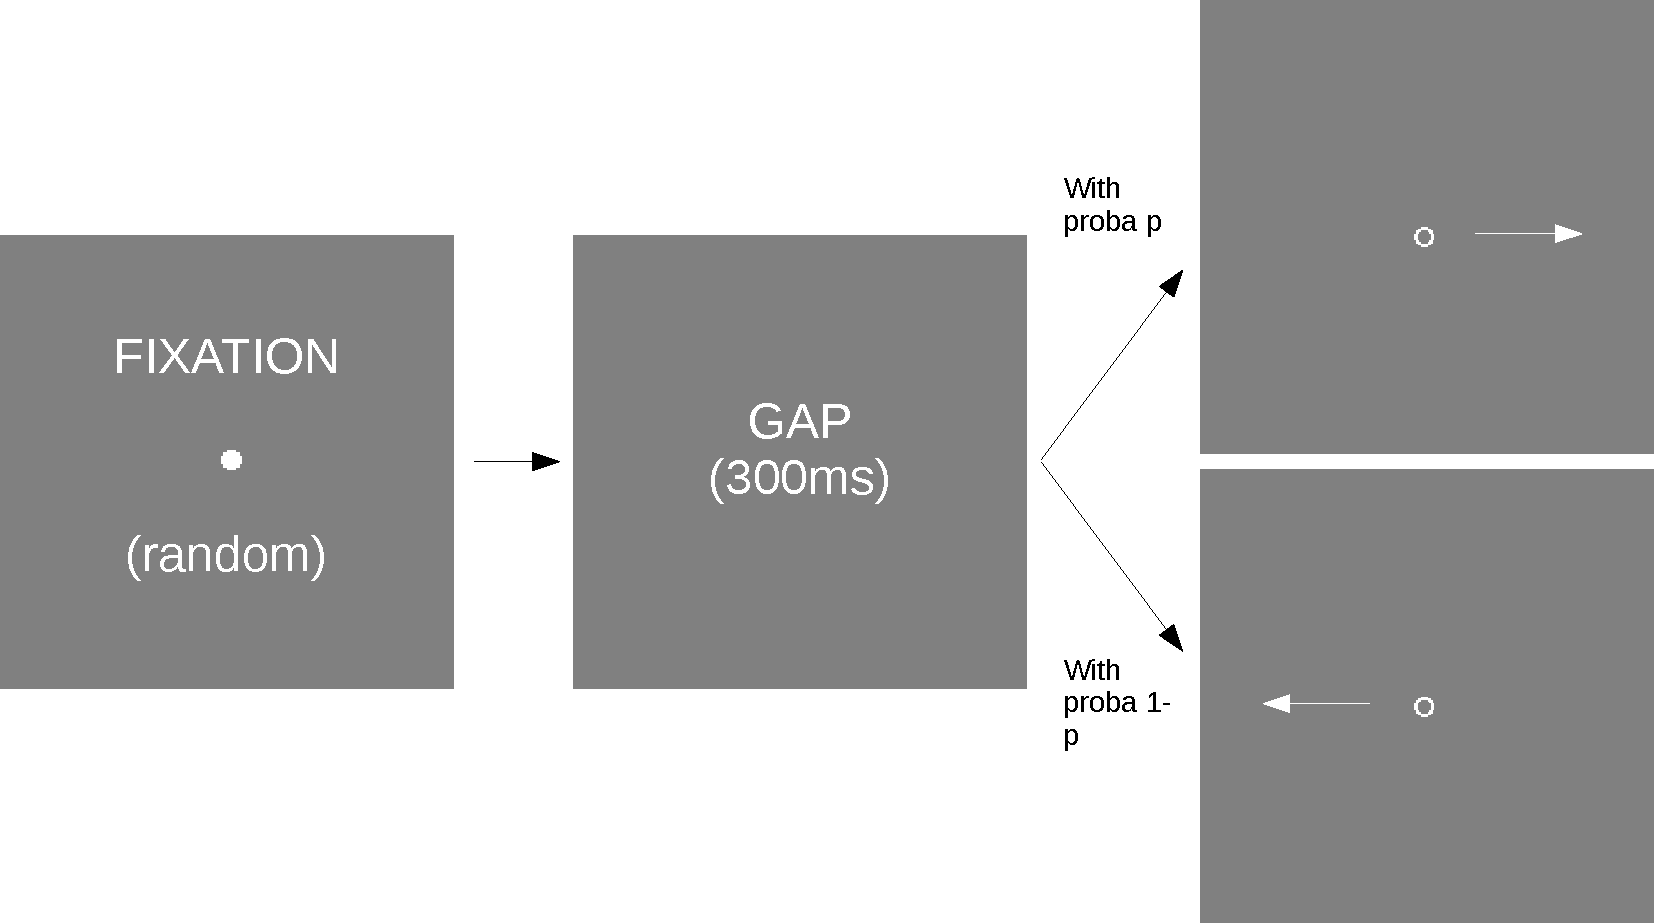
\includegraphics[width=1\linewidth]{anna_methode}
%\end{center}
\begin{tabular}{cc} 
    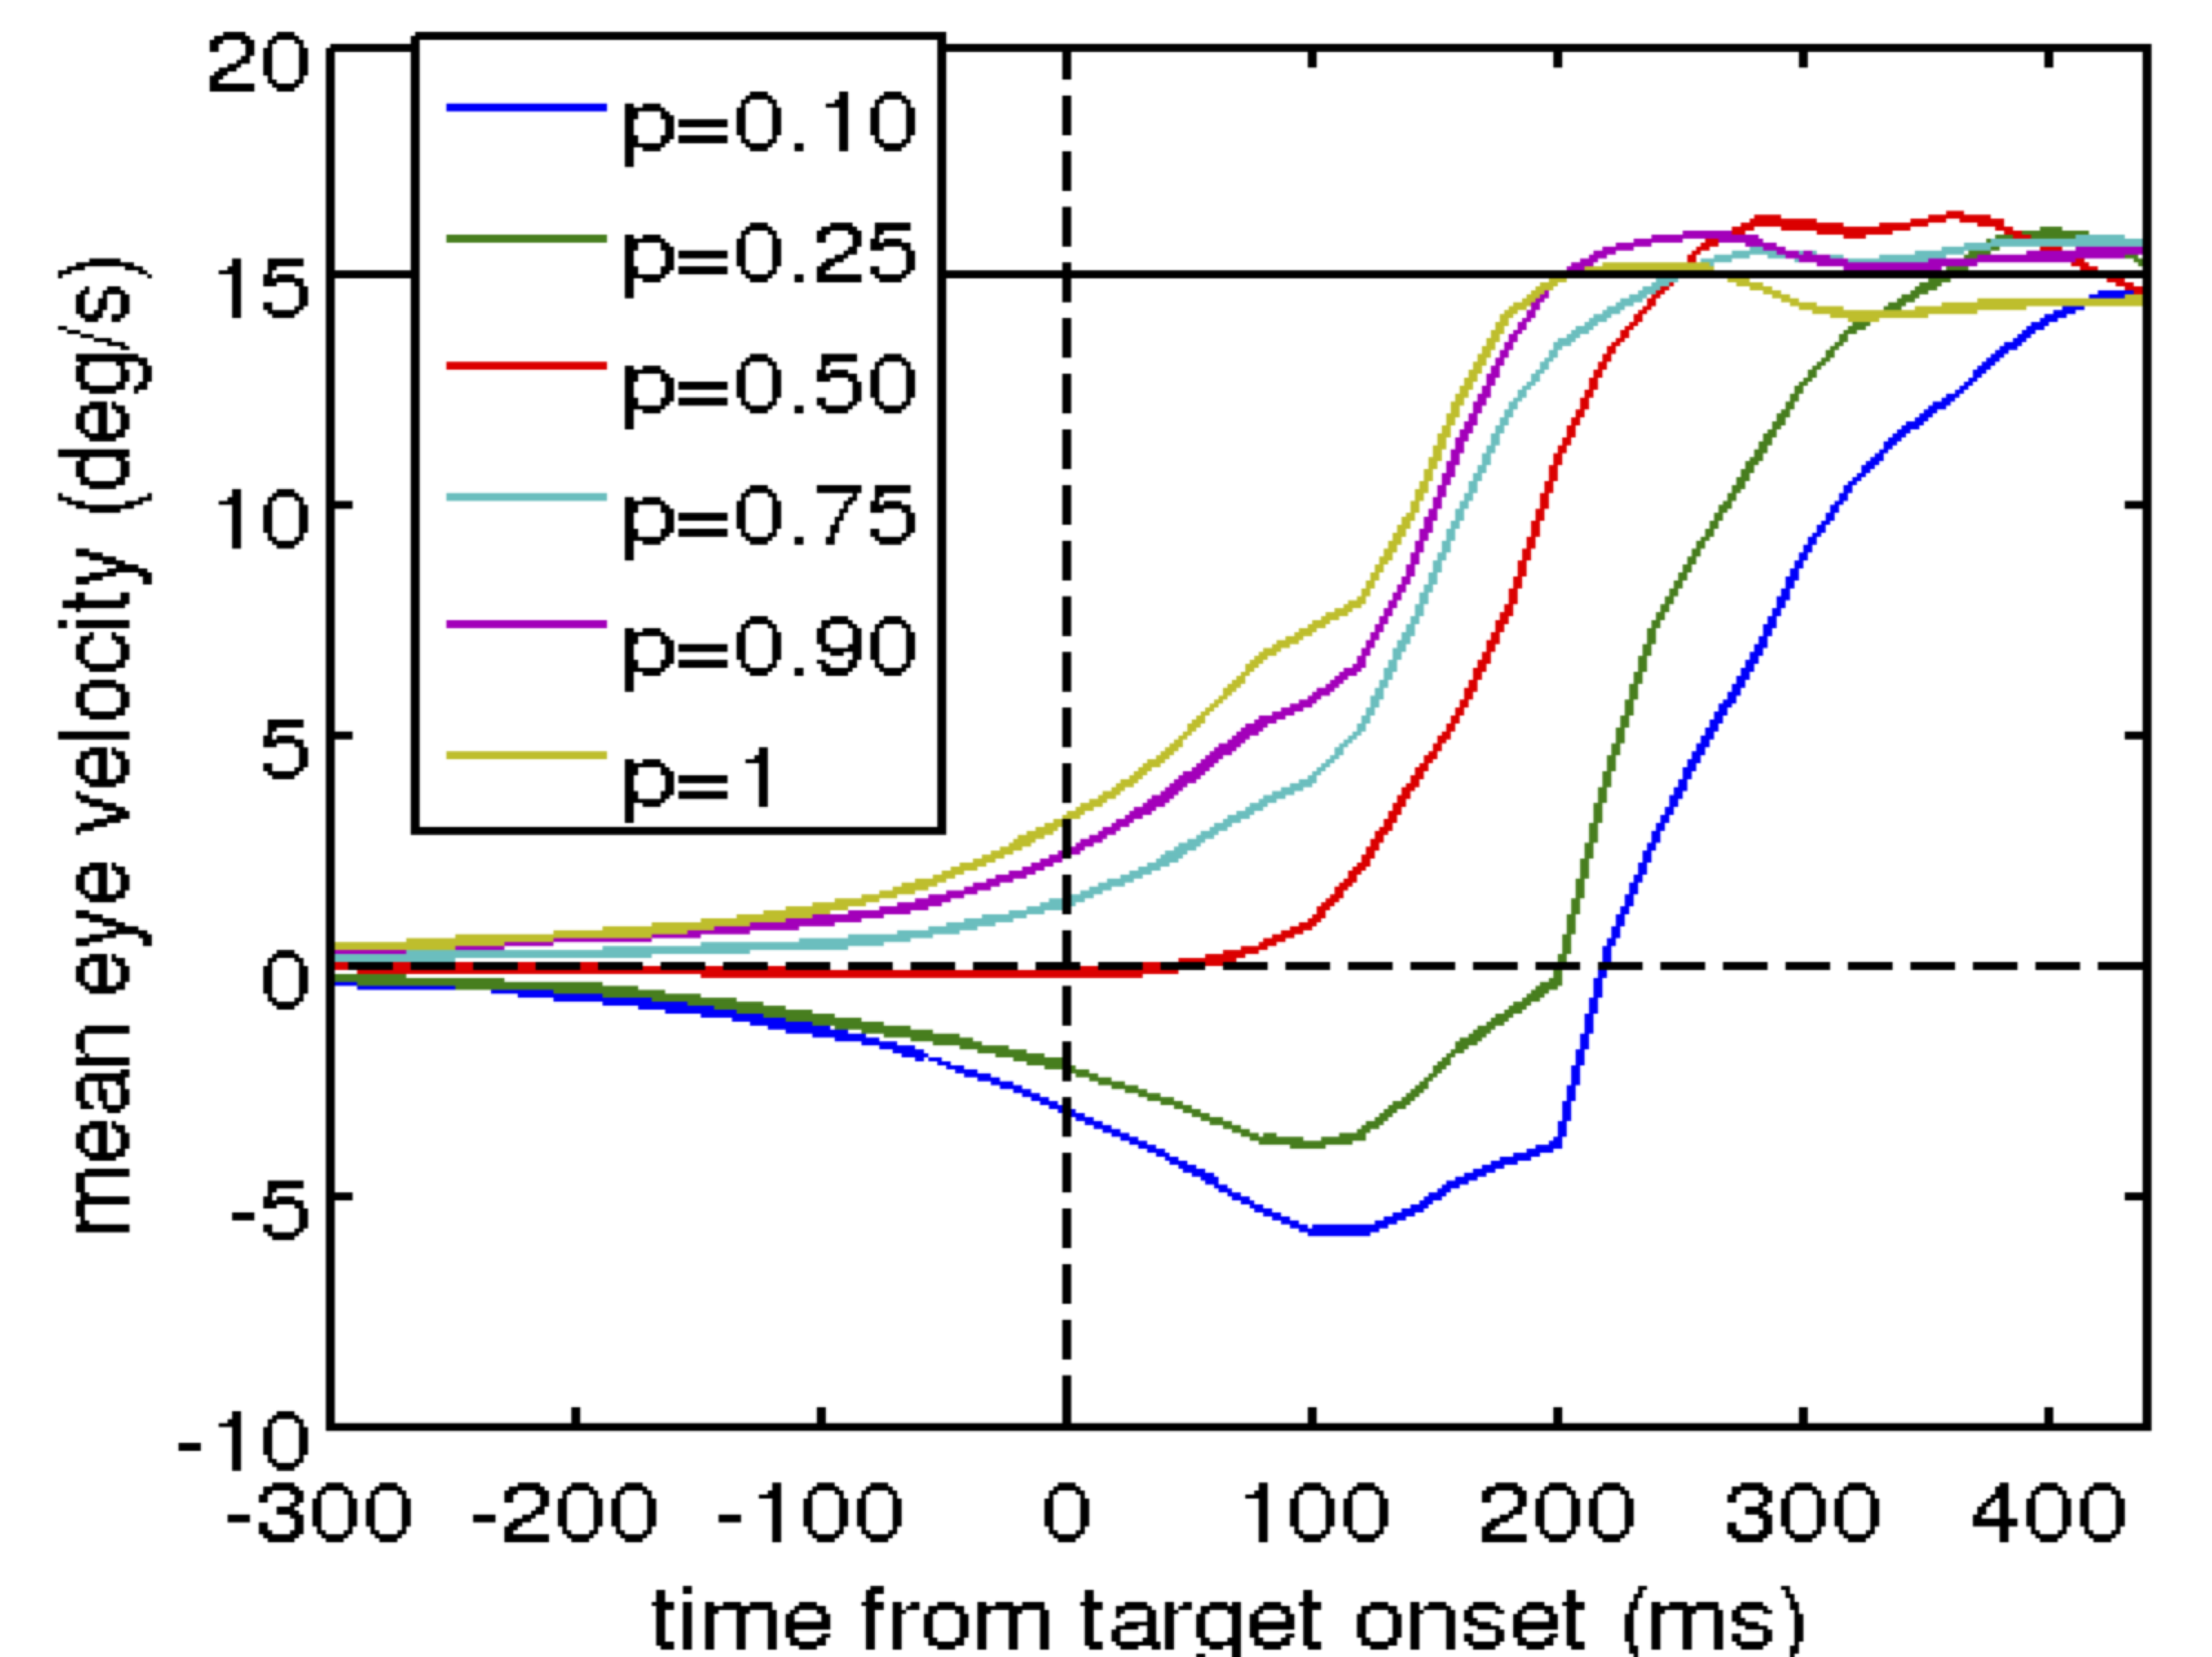
\includegraphics[width=.49\linewidth]{image_anna_1} & 	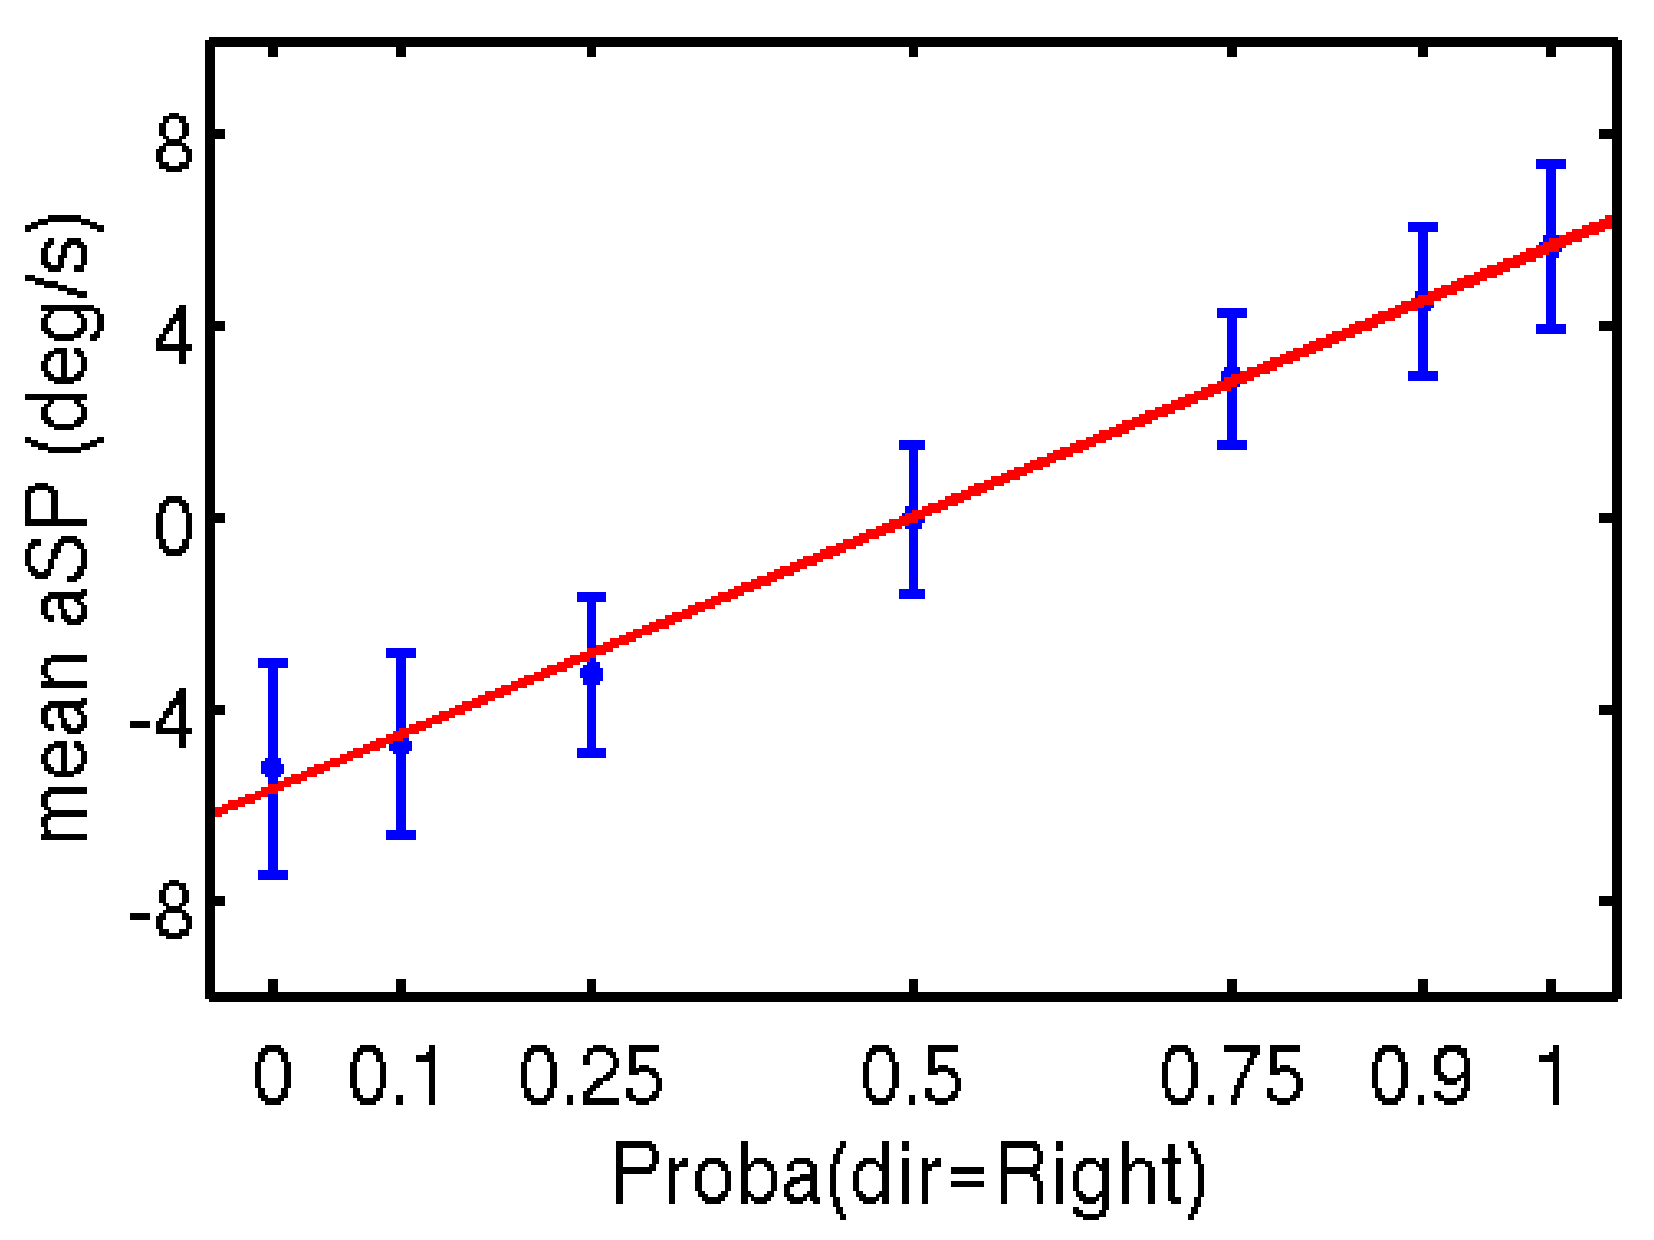
\includegraphics[width=.49\linewidth]{image_anna_2}
\end{tabular}
%\vspace{0.5cm}
%\begin{center}
%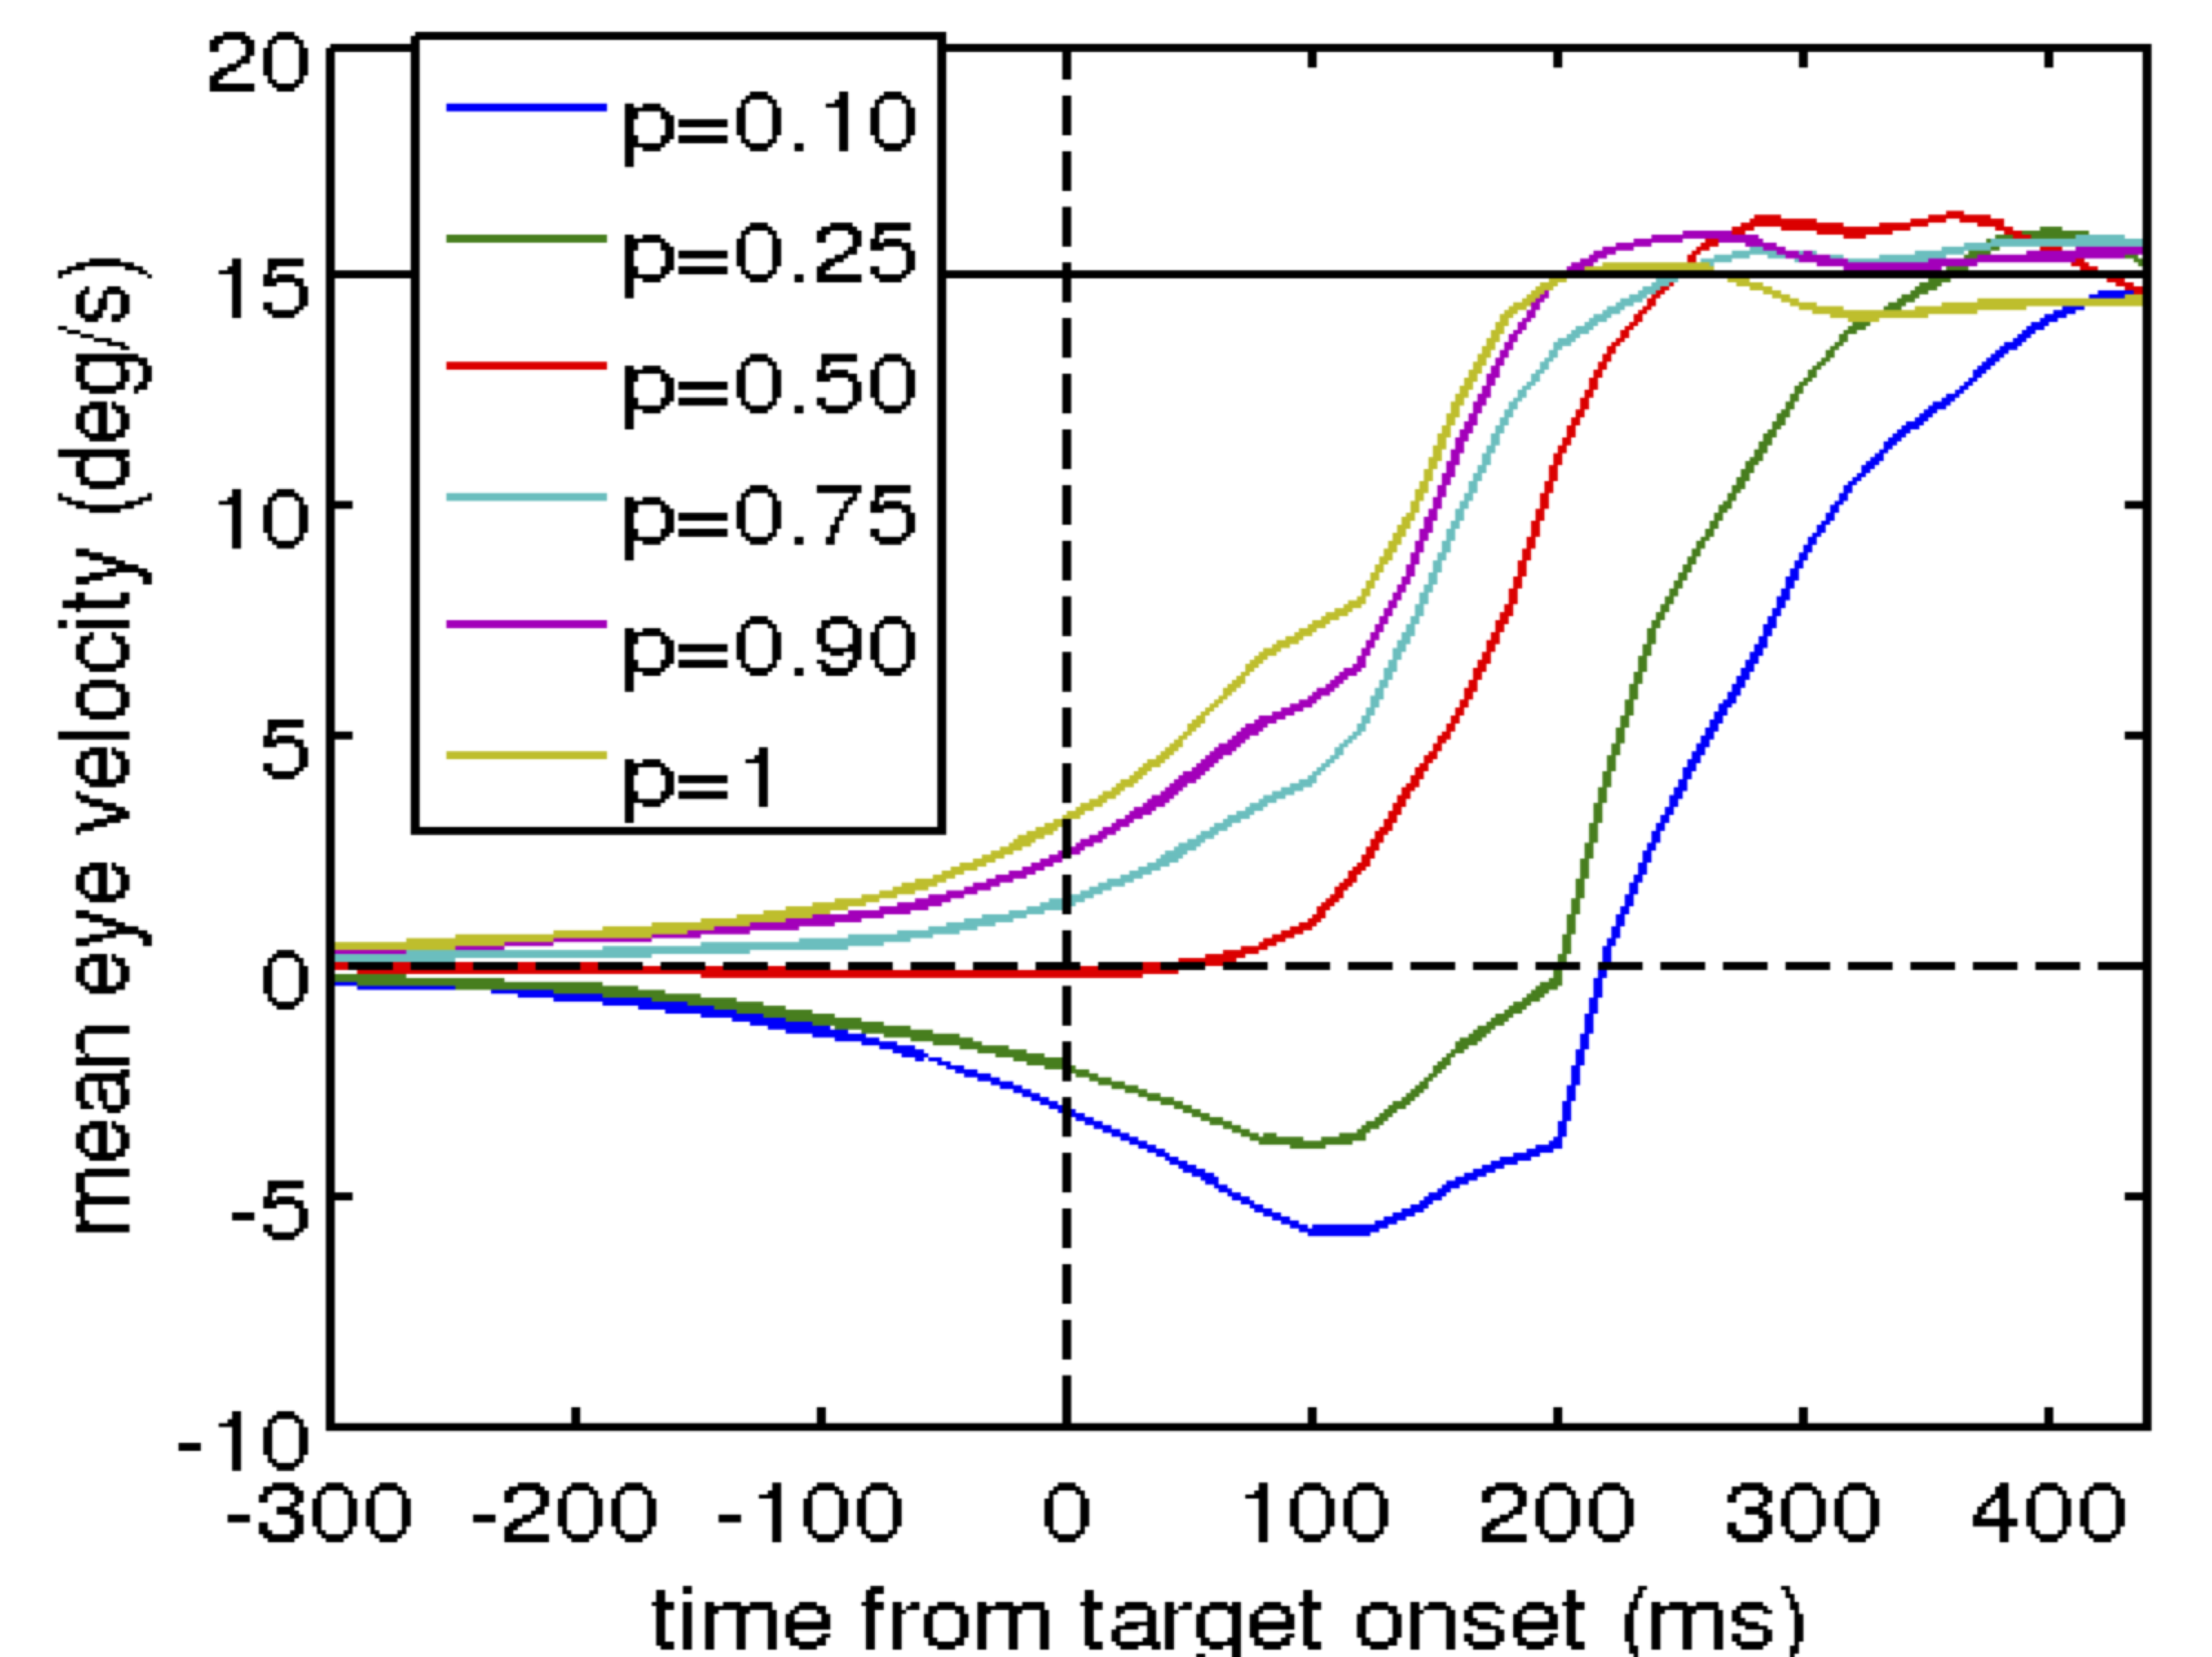
\includegraphics[width=0.9\linewidth]{image_anna_1}
%\end{center}
%\vspace{0.5cm}
%\begin{center}
%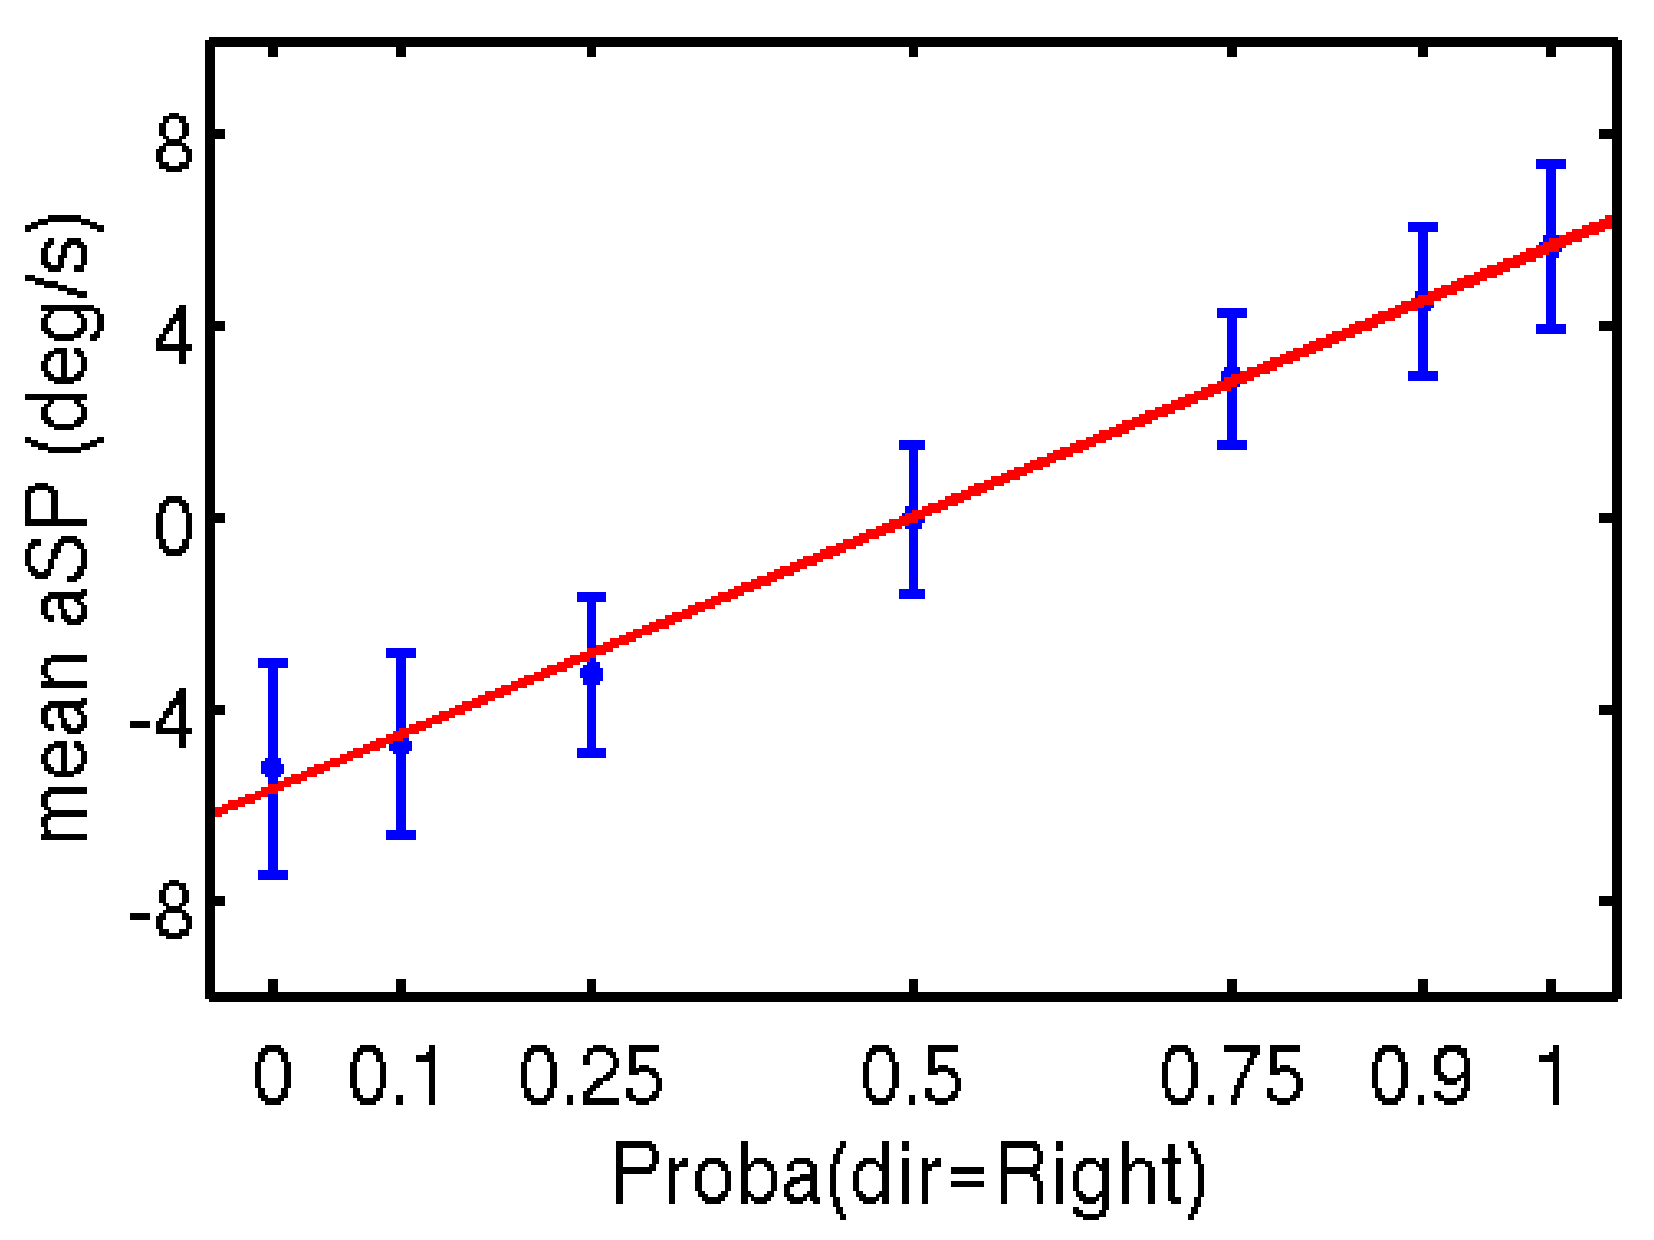
\includegraphics[width=0.9\linewidth]{image_anna_2}
%\end{center}
\caption{\emph{Anticipatory SPEM (aSPEM): psychophysics and results} %
%: TODO présente sur 3 colonnes: 1/  le protocole 2/ les résultats sur du fixed block length 3 / la généralisqation qu'on veut faire ici : random-length + bet
% cf 0_protocole.ipynb
% cf https://github.com/chloepasturel/AnticipatorySPEM/issues/19
\textbf{(A)} Human observers were presented $200$ trials which consists of sequentially: a fixation dot (random duration), a blank screen (fixed duration of XXX ms) and a moving dot (XXX 20 deg/s) which the observers were instructed to follow. The direction of the dot was drawn pseudo-randomly
\textbf{(B)} Average velocity traces of eyes. One can distinguish two phases: a visually driven component (after a latency of...) and also an anticipatory part where for ...
\textbf{(C)} In this paper, we extended the experiment by asking to the observer on a subsequent day, but with the same sequence to rate the level of confidence for their estimate of the direction of the dot before each trial.
 }
\label{fig:intro}
\end{figure}
%-------------------------------------------------------------%


However, such estimate may become particularly challenging in a dynamic context, where the probabilistic contingencies vary in time in an unpredictable way. In addition, whether and how the information processing underlying the buildup of aSPEM is linked to an explicit estimate of probabilities is unknown.

%: outline

extension of BCP to binomial data + python implementation 
psychophysics on eye movements (reflex / cognitive) => generalization of previous results
analysis of inter-individual changes


%: %%%%%%%%%%%%%%%%%%%%%%%%%%%%%%%%%%%%%%%%%%%%%%%%%%%%%%%%%%%%%%%
\section{Material and Method}

\subsection{Forgetful-agent model (Leaky integrator)}
% it's a particular case of the solution to the generative model assumaing a fixed -block length
%
% Following the~\citet{Maus2015} analysis, we performed a first study~page~\pageref{chap:4} in which we wanted to test a more realistic model of how trial-history shapes motion expectation in a direction-biased experiment.  According to~\citet{Anderson2006}, the temporal evolution for the expectation of a given event can be modeled making a simple assumption: the update of the estimated probability for an event is based on the discount of the previous estimated probability by a factor$~\lambda$, relative to new information. The value of$~\lambda$ presumably represents a compromise between responding rapidly to genuine changes in the environment and not prematurely discarding information still of value for slowly changing contexts. We extended~\citet{Anderson2006}'s approach to our analysis of anticipatory smooth pursuit across different contexts corresponding to the experimental blocks with different global probability-bias. We designed a forgetful agent estimating the target motion direction-bias according to the following iterative equation, where the estimated probability of a target moving rightwards is obtained from (1) the previous bias inference, (2) the imposed target directions and (3) a memory decay in the weighting of information. This model can be explained with the following equation:
%
%
%\[\hat{p}_{0} = 0.5\]
%\[\hat{p}_{i+1} = (1 - 1/\tau)*\hat{p}_{i} + 1/\tau * \textit{D}_{i}\] 
%
%where
%\begin{enumerate}[label={}]
%\item $\hat{p}_{i}$ = estimation of rightward trials probability at trial~\textit{i}
%\item $\tau$ = characteristic memory decay time (in trials for the inference of $p$)
%\item $\textit{D}_{i}$ = Imposed directions. Sequence of 0 (leftward) and 1 (rightward) trials
%\end{enumerate}
%
% We simulated the sequence of p-estimates of the forgetful agent for each direction-bias block and for different values of~$\tau$. Fig~\ref{fig:p_est.pdf} below illustrates, for the $p=90\%$ direction bias block, the intuitive notion that with a small value for~$\tau$~(or equivalently a volatile memory) the agent's estimate is more sensitive to changes in the target direction trial sequence. On the other hand,  with larger~$\tau$~like 40 or 50, the estimation of p tends to fluctuate only very mildly around the global direction-bias over the experimental block.
%
%\begin{figure}[H]
%\centering
%\begin{subfigure}{1\textwidth}
%\includegraphics[width=1\textwidth]{p_est.pdf}
%\phantomcaption{\label{fig:p_est.pdf}}
%\end{subfigure}
%\caption[A forgetful-agent]{The forgetful agent's $p$-estimations with different values of~$\tau$ for the $p=90\%$ direction-bias block\label{fig:p_est.pdf}}
%\end{figure}
%
% Then, we performed a linear regression analysis of the relation between the experimentally measured anticipatory eye velocity and the simulated estimate of p for each direction-bias block. To do so, we again pooled together the eye movement velocity from all participants in each experimental condition and along the direction-bias estimated by the model at the time of their triggering. We then estimated the correlation coefficient $R$ as a function of~$\tau$. We found that $R$ is maximised for~$\tau = 5$ in $p = 50\%$ blocks ($R=.18$, $p<.05$) and $p = 75\%$ blocks ($R=.27$, $p<.05$) , and for~$\tau = 10$ for $p = 90\%$ blocks ($R=.32$, $p<.05$) (see Fig~\ref{fig:R_BL.pdf}). The correlation coefficient decreases for higher values of~$\tau$, coherent with the previous study from~\citet{Maus2015} from which we inspired this analysis. Still, the overall $R$ values are slightly higher compared to the raw linear regression with the unweighted fixed-size memory, indicating a better performance of this "forgetful" agent model. 
%
%\begin{figure}[H]
%\centering
%\begin{subfigure}{1\textwidth}
%\includegraphics[width=1\textwidth]{R_BL.pdf}
%\phantomcaption{\label{fig:R_BL.pdf}}
%\end{subfigure}
%\caption[Pearson's R between experimental data and forgetful agent]{Linear regression coefficient R as a function of~$\tau$~$(1/\lambda)$ . This quantity is a rough estimate of the matching between the simulated p-estimates by the forgetful agent and experimental anticipatory eye velocity.\label{fig:R_BL.pdf}}
%\end{figure}
%
% We then looked at the linear relation of experimental data with the probability bias estimated by the model throughout all direction blocks for all our participants with~$\tau = 10$ and as we can see on Fig~\ref{fig:P_VEM_vs_pestBL.png}, we found a graded relation between Pearson's $R$ with  $R = .17$ ($p<.05$) in $p = 50\%$ blocks, $R=.27$ ($p<.05$) in $p = 75\%$ and $R=.30$ ($p<.05$) in $p = 90\%$ blocks. This shows that anticipatory smooth eye velocities are somehow related to the estimation of $p$ given by a forgetful agent. The overall computation of this analysis to all our condition showed, coherently with~\citep{Maus2015} (see study~\ref{chap:4},~page~\pageref{chap:4}), a tendency of having higher R's for short-memory, independently of the experimental condition (see Fig~\ref{fig:R_summary_2.pdf}). Though, it is important to note a better fitting quality for this using the forgetful-agent model as in~\citet{Anderson2006}.
%
%\begin{figure}[H]
%\centering
%\begin{subfigure}{1\textwidth}
%\includegraphics[width=1\textwidth]{P_VEM_vs_pestBL.png}
%\phantomcaption{\label{fig:P_VEM_vs_pestBL.png}}
%\end{subfigure}
%\caption[Anticipatory smooth velocity classified by the estimated probability bias]{Linear regression of anticipatory velocities in function of a~$\tau$~$(1/\lambda)$ = 10 estimation. \label{fig:P_VEM_vs_pestBL.png}}
%\end{figure}
%
%\begin{figure}[H]
%\centering
%\begin{subfigure}{1\textwidth}
%\includegraphics[width=1\textwidth]{R_summary_2.pdf}
%\phantomcaption{\label{fig:R_summary_2.pdf}}
%\end{subfigure}
%\caption[Relation between P-estimation and experimental conditions]{Linear regression of anticipatory velocities in function of a~$\tau$~$(1/\lambda)$ = 10 estimation for each conditions. \label{fig:R_summary_2.pdf}}
%\end{figure}
%
% To conclude on this section, the "forgetful agent" computed an exponentially-weighted moving average and estimated the probability of a stimulus going to the right given the previous instances of rightward stimulus and a progressive discount of past information. When we looked at the relation between aSPEM velocities and the direction-bias estimated by our model, we found higher Pearson's R for short-term memory ($\approx$ 5 to 10 trial history lengths) rather than long-term memory. However, a first critic could be that our proposed model may be too rigid and does not sufficiently imply the concepts of volatility~\citep{Behrens2007} or Bayesian uncertainty~\citep{Vilares2011}. It seems plausible that the memory (history length) the brain uses for inference is varying and that this variation could be related to the volatility inferred from information in the past. For instance, our model could not be applied to $p = 100\%$ rightward direction blocks because of a pretty quick saturation toward an estimation of probability equal to 1 even though experimental aSPEM datas shows a weak but existing proportion of aSPEM to the left direction. To address this hypothesis, our next model work will be inspired by a Bayesian Change-point detection model~\citep{Adams2007}, which mimics an ideal agent inferring both the likelihood of a specific event's occurrence with the volatility of the environment (e.g the duration since a change in bias).
%

\subsection{Psychophysics}



% TODO replace this with the actual protocol using psychopy

%cf. https://github.com/chloepasturel/AnticipatorySPEM/issues/19
\textbf{Stimuli were generated using PsychoPy 1.85.4 on a Mac running OS 10.6.8 (A VERIFIER) and displayed on a 20" Viewsonic p227f monitor (A VERIFIER) with resolution $1280\times 1024$ at 100~\si{\Hz} (60 ?). Psychophysics routines were written using PsychoPy 1.85.4 controlled the stimulus display. Observers sat 57~\si{\cm} from the screen in a dark room. Twelve observers (29 years old +/- 5.15) with normal or corrected-to-normal vision took part in these experiments. They gave their informed consent and the experiments received ethical approval from the Aix-Marseille Ethics Committee in accordance with the declaration of Helsinki.}


3 blocks of 200 trial - with 4 sub-blocks of 50 trials


 * the whole experiment was coded by Chloé using :
 - python for the generative model,
 - the psychopy library for the stimulus display + connection to the eyelink 1000 that we used to record EMs
 - numpy, pandas and pylab for the data analysis

  * all this code is available : for running the experiments, re-analyzing the data and doing all plots are on github

These python scripts are available at \url{https://github.com/chloepasturel/AnticipatorySPEM}.


We asked subjects to perform two tasks on different days :
%\begin{itemize}\setlength{\itemsep}{0ex}
%\item a <<Bet>>
%\item a <<recording>>
%\end{itemize}

In summary, the design of our experimental setting is therefore very similar to the previous experiment but with a more general construct:

- using the same 3-layered generative model, we generated sequences of directions

- and generated 3 blocks of 200 trials

- with an average block length of 40 trials

We anticipated that such an  experiment for which we simply recordedd the eye movements should be more difficult for observers compared to the classical experiments with longer (400 trials), fixed blocks and...

\subsection{The Bet}
In this first part, the subjects must simply answer before each trial at the question \textit{ ``How sure are you that the target will go left or right''}. This was performed by adjusting a cursor on the screen using the mouse (see Figure).

%\textbf{ Un point de fixation blanc de 10px de large est affiché au début d'un essai. Les sujets doivent ajuster le curseur sur une échelle blanche gradué placé en desous. Cette échelle présente 3 graduations : 'gauche' et 'droite' au extrémité et 'incertain' au millieu. Pour validé leurs choix, les sujets doivent cliquer sur la souris. L’échelle et le point de fixation disparaissent et une cible en mouvement à 15°/s (voir pour LB$_Bet$ 20°/s) s’affiche à l’écran. La cible est un cercle blanc mesurant 10px de large et 2px de lineWidth.}


%\textbf{Lors de cette tâche les mouvement oculaire sont enregistré à 100 Hz via Eyelink 100. Le module Python Pylink (SR research) 0.1.0 nous a permis de faire le lien entre Eyelink et nos routines python. Les sujets ont la tête fixe, et on leur demande de ne pas cligner des yeux lorsque le stimuli aparait. Chaque essais commence par la présentation d’un point de fixation blanc de 10px de large au centre de l’écran pendant une durée variable de 400 à 800 ms. Si le signal enregistré n'est pas présent dans une fenêtre de $120\times 120$ px autour du point de fixation ou si il n’est pas stable (clignement, mauvais enregistrement…), la durée de fixation recommence. À la fin de cette durée de fixation il y a un GAP de 300ms, le point de fixation disparait laissant juste un écran gris. Puis une cible en mouvement de 15°/s apparaissait de sorte que 100ms après sont apparition il soit au centre de l’écran, afin d’évité la première saccade. La cible est un cercle blanc mesurant 10px de large et 2px de lineWidth (REDONDANT).}


This is why we added a supplementary experiment for each observer but on a different day for which we asked at every trial to give a subjective, conscious evaluation of the direction of the next trial + a confidence about this inference. Once this information given by the subject, we were showing the actual outcome.

Interestingly, we used exactly the same sequence, allowing to make a direct comparison of the results of both experiments

We called this experiment the bet experiment.


\textbf{Tous les 50 essais le 'score' du sujet sur les 50 derniers essais est affiché au centre de l'écran, le sujet doit appuyer sur la barre espace du clavier pour continuer (doit dire a l'expérimentateur quand il veux continué, on ne pouvais pas brancher une souris et un clavier en même temps). Ce score est égal à $\sum_{x=0}^{50} \frac{Bet_{x} \times dir_x}{50} \times 100$. Où $Bet_x$ est le parie du sujet à chaque début d'essaie comprie entre -1 pour la gauche et 1 pour la droite, $dir_x$ est la direction de la cible pour chaque essai, -1 pour la gauche et 1 pour la droite.}


%\subsection{The Bet}
%Example of results obtained during the bet :
%\begin{center} 
%    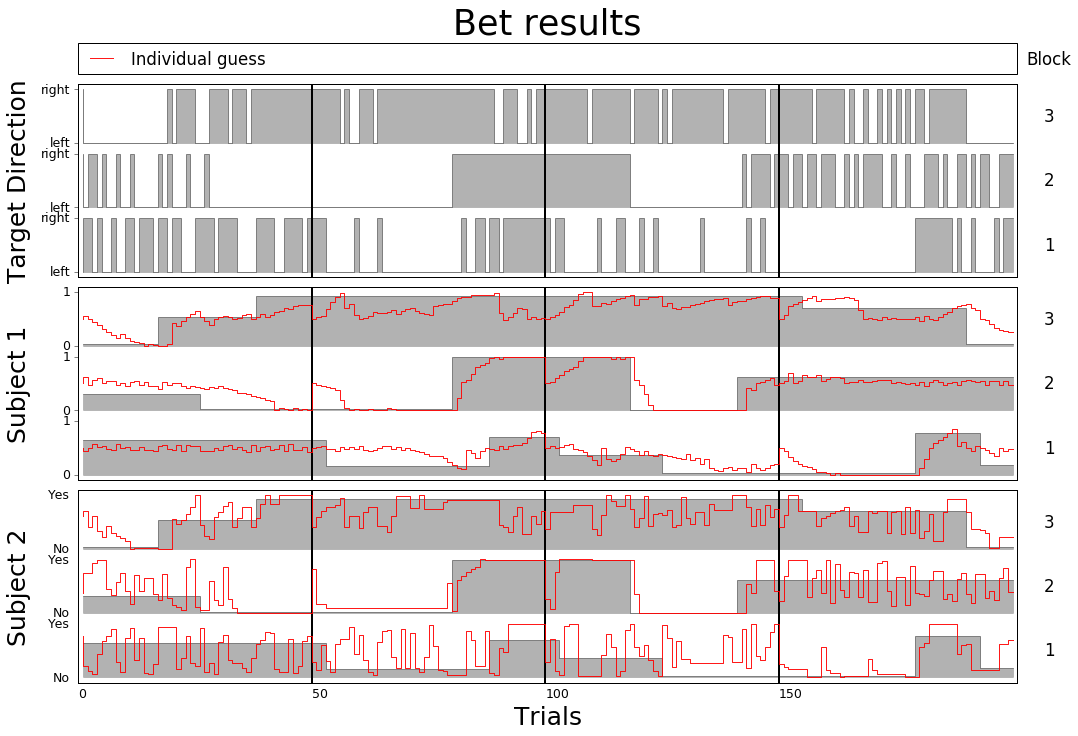
\includegraphics[width=1\linewidth]{results_pari}
%\end{center}
%%Comparison of probabilities bet with respect to the real probability :
%The scatter plot of the value of the bet (probability bet) as a function of the real probability at every given trial shows that there is a good correlation between both values:

%\begin{center}
%    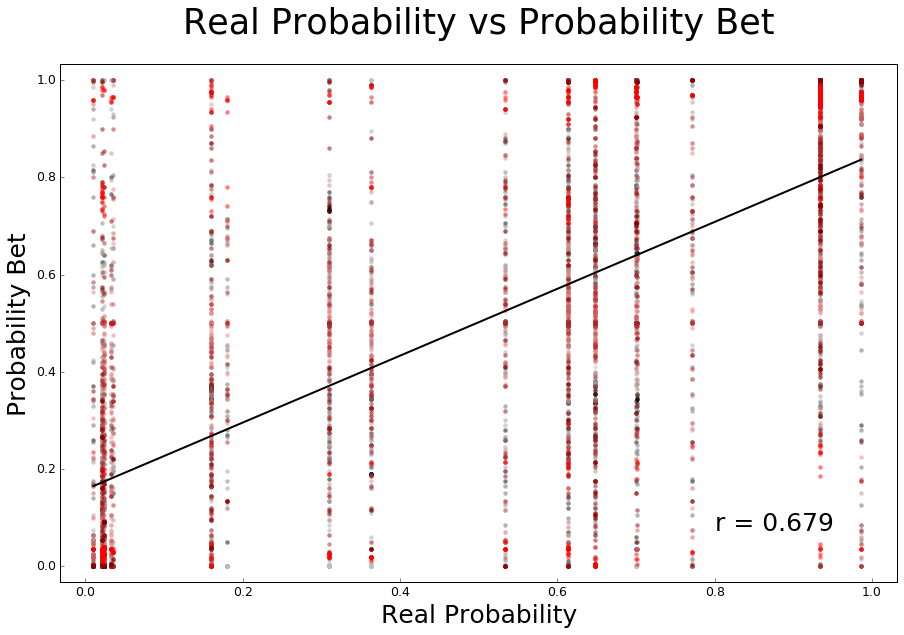
\includegraphics[width=1\linewidth]{p_real--p_bet}
%\end{center}

\subsection{Eye movements recording}
Then, we recorded their eye movements as they were tracking the target's motion. Importantly, we used that exact same sequence.

% TODO replace this with the actual protocoml using psychopy
%Stimuli were generated using Matlab 7.10.0 on a Mac running OS 10.6.8 and displayed on a 20" Viewsonic p227f monitor with resolution $1024\times 768$ at 100~\si{\Hz}. Psychophysics routines were written using Matlab and Psychtoolbox 3.0.9 controlled the stimulus display. Observers sat 57~\si{\cm} from the screen in a dark room. Six male observers with normal or corrected-to-normal vision took part in these experiments. They gave their informed consent and the experiments received ethical approval from the Aix-Marseille Ethics Committee in accordance with the declaration of Helsinki.

In parallel, we are developing new automatic routines for the advanced analysis of oculomotor traces. In order to extract the relevant parameters of the oculomotor responses (latency, gain, initial acceleration, catch-up saccades), we developed new tools based on best-fitting procedure of predefined patterns (i.e. the typical smooth pursuit velocity profile).

These python scripts are available at \url{https://github.com/invibe/ANEMO}.


\subsection{Eye movements analysis}

In order to extract the relevant parameters of the oculomotor responses, we developed new tools based on a best-fitting procedure of predefined patterns and in particular the typical smooth pursuit velocity profile that was recorded for the aSPEM (Top row). This was applied to each trial individually, and we show below some prototypical example of respectively a neutral, anticipatory positive and anticipatory negative aSPEMs examples (respectively second to bottom rows). 


%-------------------------------------------------------------%
%:  FIGURE 2 fig:results_raw
\begin{figure}%[b!]
%\vspace{2mm}
\begin{center} 
    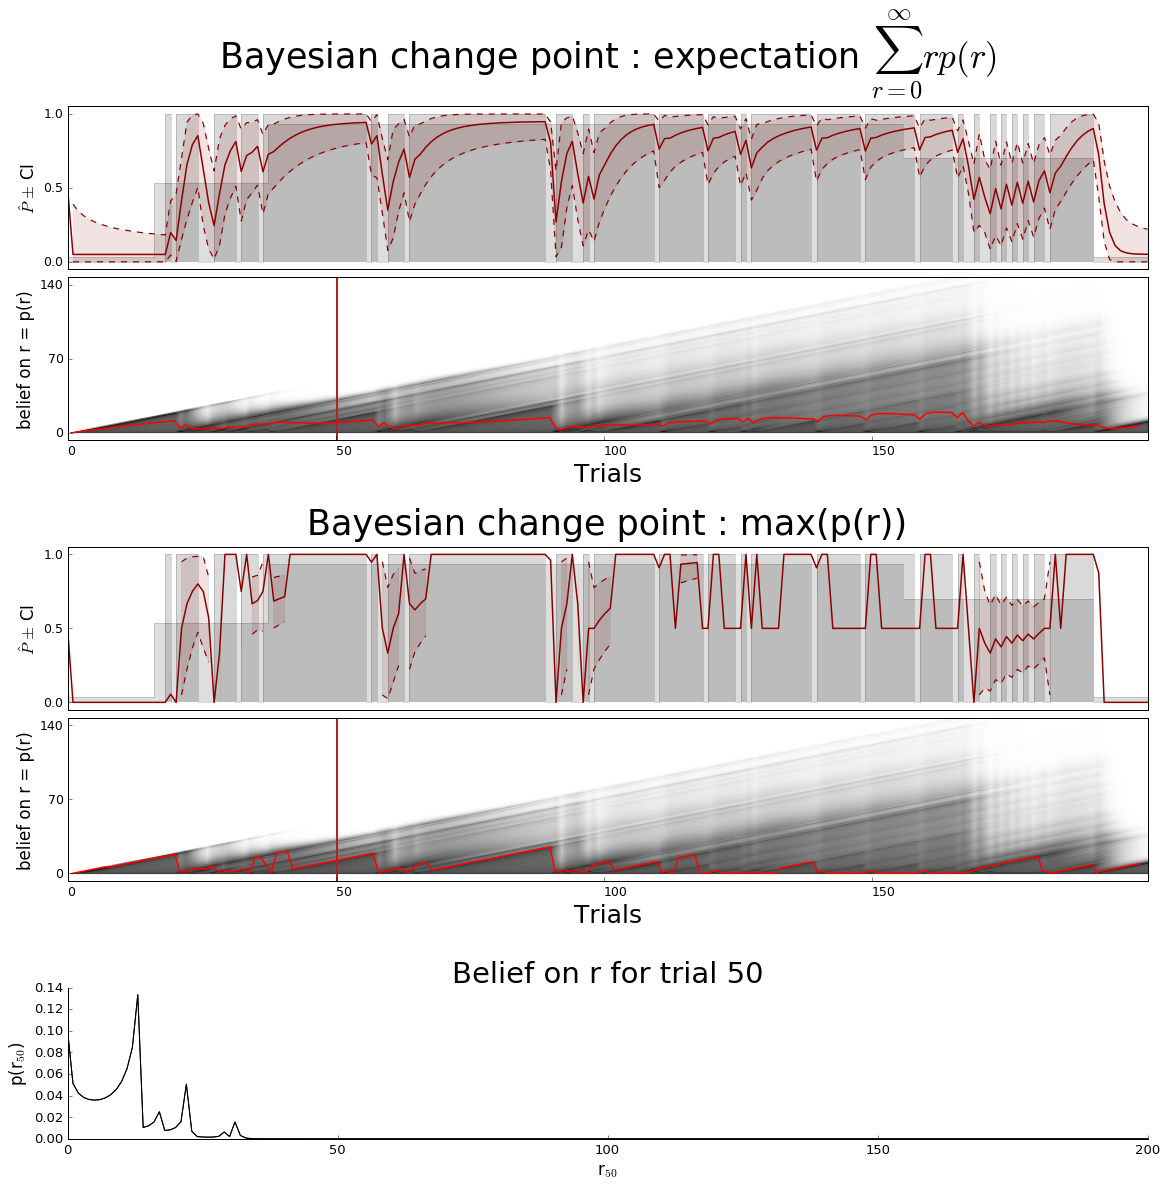
\includegraphics[width=1\linewidth]{bayesianchangepoint}
\end{center}
%: TODO présente le prtocole avec les résultats bruts pour un sujet caractéristique 
\caption{\emph{The binomial switching model and raw Psychophysical results}%
% cf 1_generative-model.ipynb
~\textbf{A} This diagram represents the stochastic model chosen to generate the sequence of directions %
% cf 3_Results_2.ipynb
~\textbf{B} Raw results for one characteristic observer. In this plot we superpose the sequence of event (red or blue dots for respectively left or right directions), the (hidden) evolution of the value of $p$ (horizontal black lines) and the underlying times for switches (vertical black lines). Note that we introduced pauses every 50 trials to prevent from fatigue. Using a pseudo-random number generator with the same seed, we could present the exact same sequence to all subjects. %
We have superposed the trace of 1/ the aSPEM strength as measured by the horizontal displacement at the onset of the visually-driven SPEM, 2/ the response to the bet experiment and 3/ the result of the BCP model. 
}
\label{fig:results_raw}
\end{figure}
%-------------------------------------------------------------%
%%-------------------------------------------------------------%
%%: fig:eye_fits
%\begin{figure}%[b!]
%%\vspace{2mm}
%\begin{center} 
%    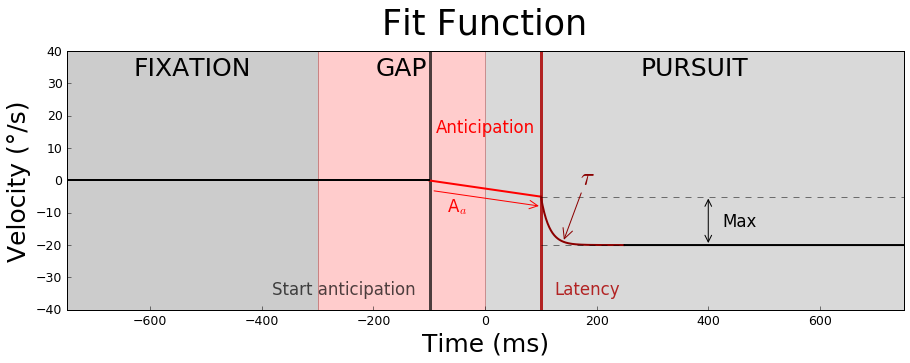
\includegraphics[width=1\linewidth]{Fonction_Fit}
%    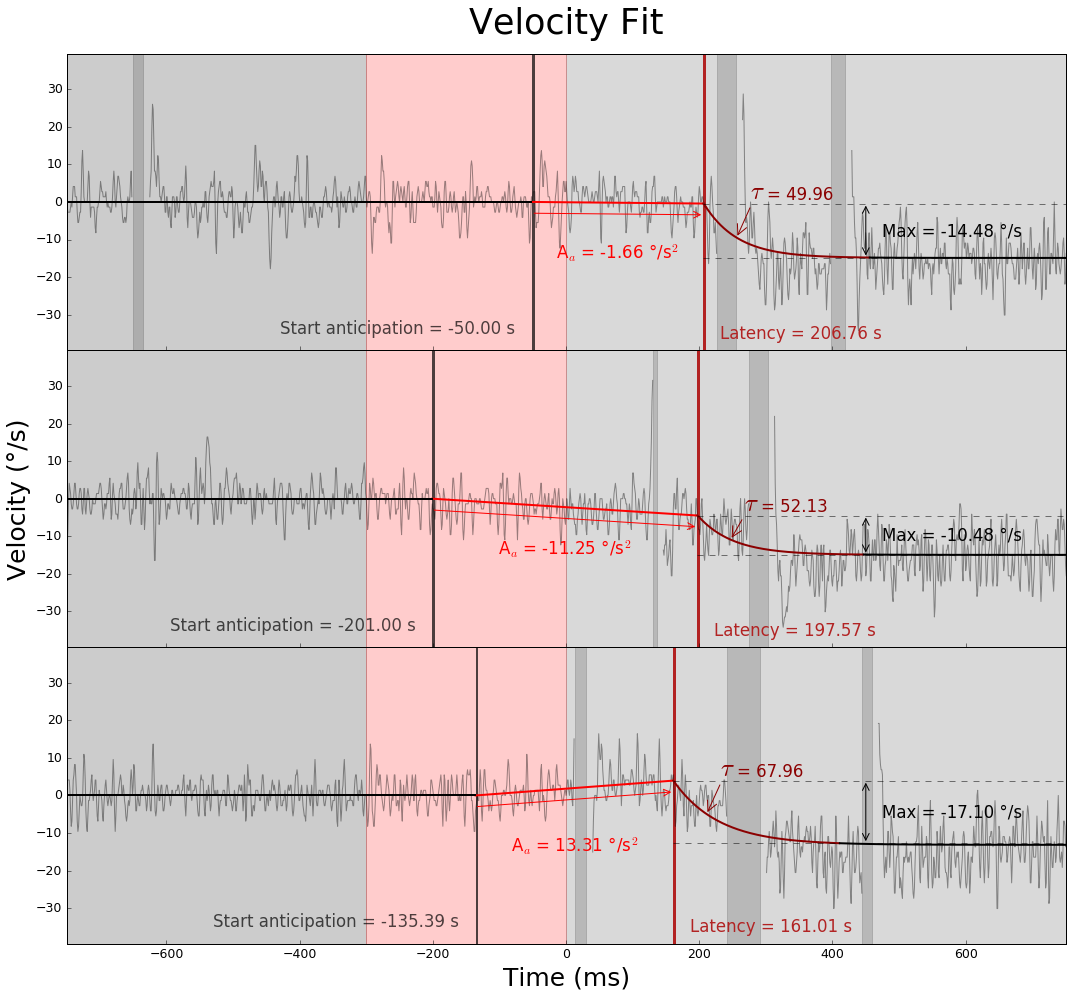
\includegraphics[width=1\linewidth]{Fit_vitesse}
%\end{center}
%\caption{\emph{Eye movements analysis} \textbf{(A)} 
%\textbf{(B)} 
%\textbf{(C)}  }
%\label{fig:eye_fits}
%\end{figure}
%%-------------------------------------------------------------%
%
%: %%%%%%%%%%%%%%%%%%%%%%%%%%%%%%%%%%%%%%%%%%%%%%%%%%%%%%%%%%%%%%%
\section{Results: Bayesian change point model}

% These python scripts are available at \url{https://github.com/laurentperrinet/bayesianchangepoint}.
%TODO include changing point theory and bibliography
% TODO : check http://www.princeton.edu/~rcw2/papers/WilsonEtAl_PLOSCompBiol2013.pdf and bernouilli case + evaluation


\subsection{Bayesian change point model}

We have designed an agent adapted the Bayesian Online Change-point Detection model~\parencite{AdamsMackay2007}. This model uses a latent variable r which represents the length of the current interval during which motion-direction probability ($\hat{P}$) has not changed. The agent infers at each trial the likelihood  of r and then deduces the optimal $\hat{P}$ (we used the expected value and the max as readouts) and the uncertainty associated to it. We simulated the model across our experimental sequences, as illustrated by the example for the third block.


* an implementation of
[Adams &amp; MacKay 2007 "Bayesian Online Changepoint Detection"](http://arxiv.org/abs/0710.3742)
in Python.

````
@TECHREPORT{ adams-mackay-2007,
AUTHOR = "Ryan Prescott Adams and David J.C. MacKay",
TITLE  = "Bayesian Online Changepoint Detection",
INSTITUTION = "University of Cambridge",
ADDRESS = "Cambridge, UK",
YEAR = "2007",
NOTE = "arXiv:0710.3742v1 [stat.ML]",
URL = "http://arxiv.org/abs/0710.3742"
}
````

* adapted from https://github.com/JackKelly/bayesianchangepoint by Jack Kelly (2013) for a binomial input.

* This code is based on the  [MATLAB implementation](http://www.inference.phy.cam.ac.uk/rpa23/changepoint.php) provided by Ryan Adam. Was available at http://hips.seas.harvard.edu/content/bayesian-online-changepoint-detection

 * full code @ https://github.com/laurentperrinet/bayesianchangepoint


%-------------------------------------------------------------%
%:  FIGURE 3 fig:bayesianchangepoint									
%: TODO présente le principe de l'algorithme, le résultat sur une séquence et une aanlyse quantitative qui permettra de l'utiliser pour les expériences psycho
\begin{figure}%[b!]
\begin{center} 
% cf 3_Results_2.ipynb
    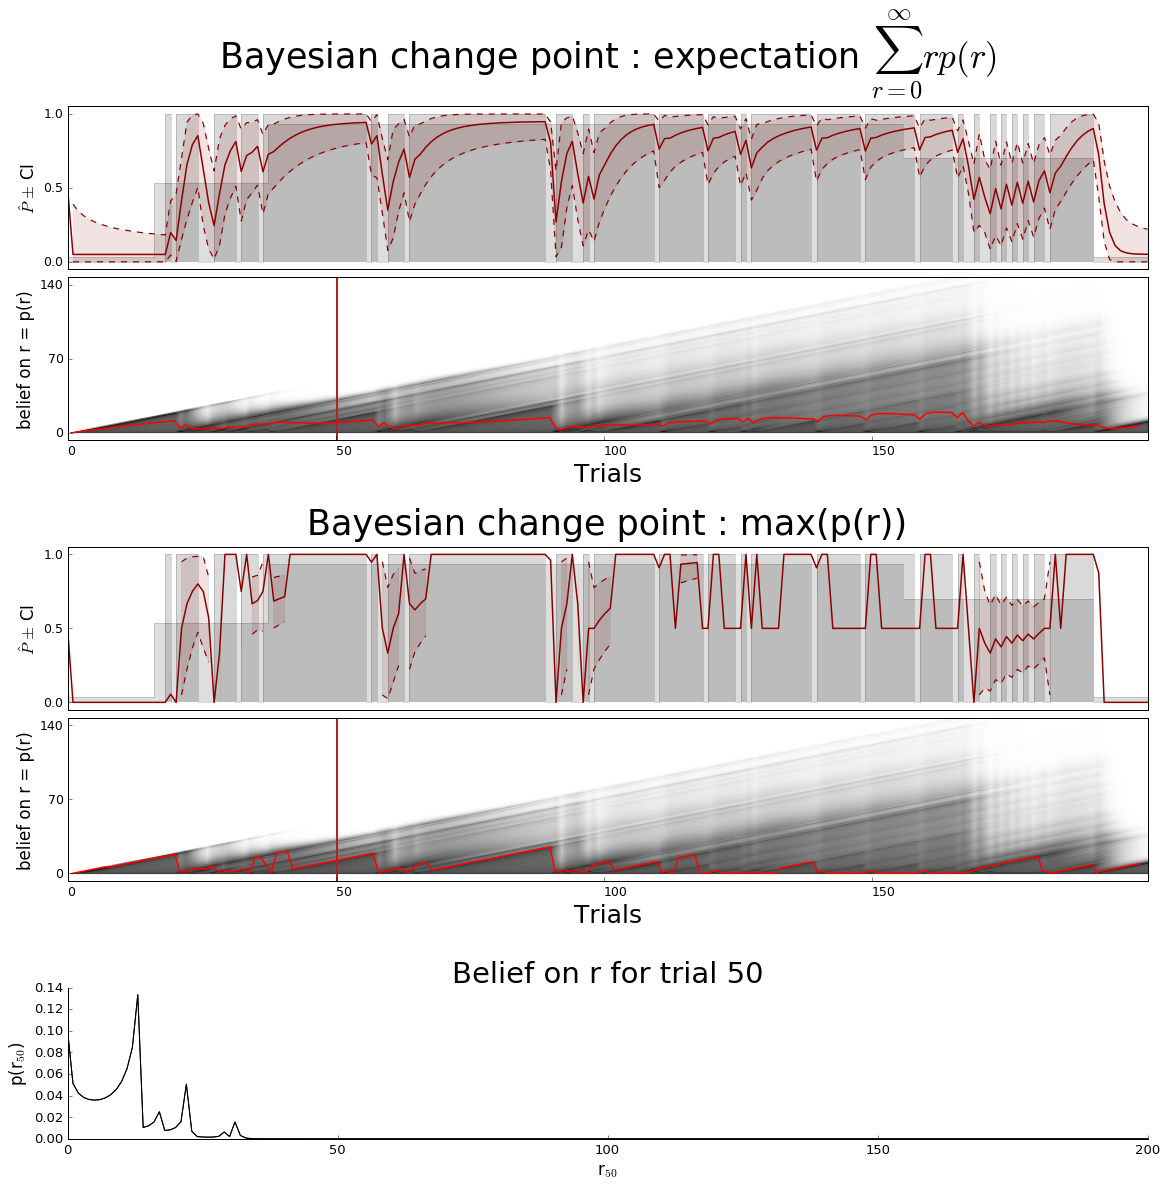
\includegraphics[width=1\linewidth]{bayesianchangepoint}
\end{center}
\caption{\emph{Bayesian change point model}~\textbf{A} shows hypothetic datas that works as a binomial choice, either 0 (leftward) or 1 (rightward). In particular, the probability switched at trials 6 and 10.~\textbf{B} shows the graph (treillis) on which the message indicates that mass probability is being passed. Black lines denotes "upwards", that is, for which there is a progression of the run length at the next step. The red line stands for the possibility that a switch happened, and then falls back to zero. The black curve stands for the run length of simulated datas in~\textbf{A} in function of time (r$_t$). We can see that the run length drops back to zero when change occurs at trials 6 and 10. \textbf{(C)}  


* in this graph information will be represented at different nodes. each node represent a belief which takes the form of a probability distribution over the set of parameters that we wish to describe.
* it can be the mean and variance of a Gaussian, but in general it will be 2 parameters. in our case, we wish to estimate p (between zero and one) - it is characterized by the beta distribution (mathematically it is the conjugate of the bernouilli distribution)
* (mathematically, we will use th family of exponenetial distributions:, gaussians, binomials) among which the beta distribution belongs
First, we initialize the first node to prior values
* at trial zero, there is no information, so we intiialize to the prior values
% use p log p + (1-p) log (1-p ) as in logistic regression?
}
\label{fig:bayesianchangepoint}
\end{figure}
%-------------------------------------------------------------%


Fig~\ref{fig:BCP_figA}~\textbf{A} shows one instance of a sequence of simulated datas of leftward and rightward trials with a probability $p$ of being rightward with possible variations through times. It also shows the predicted probability $\hat{p}$ by using the BCP algorithm. Fig~\ref{fig:BCP_figB} illustrates the belief r on the predicted probability $\hat{p}$ at a given trial. On Fig~\ref{fig:BCP_figC} and Fig~\ref{fig:BCP_figD}, we can see the belief on the run length estimation. 
 
Note, the fixed-length is imply implemented by a (broken) line with fixed run-length $r_t=\tau$) - this allows for a simple comparison 

\subsection{Bayesian change point algorithm}

%cf p33 de 2018-02-12 journal club bayesian changepoint chloe.pdf 

% Fig~\ref{fig:BCP_figA}~\textbf{A} shows one instance of a sequence of simulated datas of leftward and rightward trials with a probability $p$ of being rightward with possible variations through times. It also shows the predicted probability $\hat{p}$ by using the BCP algorithm. Fig~\ref{fig:BCP_figB} illustrates the belief r on the predicted probability $\hat{p}$ at a given trial. On Fig~\ref{fig:BCP_figC} and Fig~\ref{fig:BCP_figD}, we can see the belief on the run length estimation. 
% 
%\begin{figure}[H]
%\centering
%\begin{subfigure}{1\textwidth}
%\includegraphics[width=1\textwidth]{BCP_fig.pdf}
%\phantomcaption{\label{fig:BCP_figA}}
%\end{subfigure}
%\begin{subfigure}{0\textwidth}
%\includegraphics[width=1\textwidth]{BCP_fig.pdf}
%\phantomcaption{\label{fig:BCP_figB}}
%\end{subfigure}
%\begin{subfigure}{0\textwidth}
%\includegraphics[width=1\textwidth]{BCP_fig.pdf}
%\phantomcaption{\label{fig:BCP_figC}}
%\end{subfigure}
%\begin{subfigure}{0\textwidth}
%\includegraphics[width=1\textwidth]{BCP_fig.pdf}
%\phantomcaption{\label{fig:BCP_figD}}
%\end{subfigure}
%\caption[Bayesian Change Point model computation]{~\textbf{A} is a sequence of points representing leftward (0) of rightward trials (1) with a given probability $p$ of being rightward and that changes at some trials (clear red). The predicted probability $\hat{p}$ ($\tau=N_{trial}/4$ tells the BCP that the probability is more susceptible to change every $N_{trial}/4$), continue and dotted dark red lines shows the $p$$-$estimation.~\textbf{B} shows the probability of the run length, the probability of the having same probability consecutive trials. The red line represents the $\hat{r}$, that represents the sum of he products of each r (number of consecutive trials having the same probability)  $\sum_{r=0}^\infty r \cdot P(r)$.~\textbf{C} represent the probability of each r for trials 50 and 250 along their $\hat{r}$ and their $\hat{p}$. For instance, for trial 50, we can observe that $\hat{r}$ is close from the real number of trials during the probability has not change (real $p$ stayed for 50 trials). $\hat{p}$ is also pretty close from the real $p$ ($p=1$).~\textbf{D} shows that at trial 250 $\hat{r}$ is more far than the real r that is also equal to 50 trials. But here, $\hat{p}$ is closer from $p$ that is equal to 0.75. \label{fig:BCP_fig.pdf}}
%\end{figure}
%
% We adapted this model to the data our first study,~page~\pageref{chap:4}, by taking the alternating output of leftward/rightward trials as the sequence of observations that will be under the analysis of the model. This model uses a latent variable r which represents the length of the current interval during which motion$-$direction probability~($\hat{p}$)~has not changed. The agent infers at each trial the likelihood of r and then deduces the optimal~$\hat{p}$~(we used the expected value and the max as readouts) and the uncertainty associated to it. Finally, the whole algorithm simplifies to the following iterations:

Following the principle of Active Inference,
To summarize, the algorithm % uncover progressively

\begin{enumerate}
	\item     Initialize

	\begin{itemize}
		\item    $P(r_0)= S(r)$ or $P(r_0=0)=1$ and
		\item    $\nu^{(0)}1 = \nu_{prior}$ and $\chi^{(0)}1 = \chi_{prior}$
	\end{itemize}

	\item    Observe New Datum $x_t$
    \item    Evaluate Predictive Probability $\pi_{1:t} = P(x |\nu^{(r)}_t,\chi^{(r)}_t)$
    \item    Calculate Growth Probabilities $P(r_t=r_{t-1}+1, x_{1:t}) = P(r_{t-1}, x_{1:t-1}) \pi^{(r)}_t (1-H(r^{(r)}_{t-1}))$
    \item    Calculate Changepoint Probabilities $P(r_t=0, x_{1:t})= \sum_{r_{t-1}} P(r_{t-1}, x_{1:t-1}) \pi^{(r)}_t \cdot H(r^{(r)}_{t-1})$
    \item    Calculate Evidence $P(x_{1:t}) = \sum_{r_{t-1}} P (r_t, x_{1:t})$
    \item    Determine Run Length Distribution $P (r_t | x_{1:t}) = P (r_t, x_{1:t})/P (x_{1:t}) $
    \item    Update Sufficient Statistics :
	\begin{itemize}
		\item    $\nu^{(0)}_{t+1} = \nu_{prior}$, $\chi^{(0)}_{t+1} = \chi_{prior}$
		\item    $\nu^{(r+1)}_{t+1} = \nu^{(r)}_{t} +1$, $\chi^{(r+1)}_{t+1} = \chi^{(r)}_{t} + u(x_t)$
	\end{itemize}

    \item    Perform Prediction $P (x_{t+1} | x_{1:t}) = P (x_{t+1}|x_{1:t} , r_t) P (r_t|x_{1:t})$
    \item    go to (2)
\end{enumerate}


where $\KL{\hat p}{p}$ is the Kullback-Leibler divergence between samples $\hat p$ and model $p$ under a Bernouilli distribution
\begin{equation}
\KL{\hat p}{p} = \hat{p} \log\pa{\frac{\hat p}{p}} + (1-\hat p) \log\pa{\frac{1-\hat p}{1-p}}.
\end{equation}


Contrary to the forgetful-agent model where~$\tau$ was a fixed parameter, the BCP use a changing~$\tau$ parameter. In the latter the~$\tau$ parameter informs the BCP model that the probability is suspected to change every~$\tau$ trials. As we can see on~\ref{fig:search_tau.png}, participants do not have the same pattern of responses (examples of participants 16 and 18 below). Still we were able to extract the parameter~$\tau$ that maximizes the fit between the probability computed by the BCP model ($\hat{p}$) and the experimental datas.

%\begin{figure}[H]
%\centering
%\begin{subfigure}{1\textwidth}
%\includegraphics[width=1\textwidth]{search_tau.png}
%\phantomcaption{\label{fig:search_tau.png}}
%\end{subfigure}
%\caption[Correlation maximization in function of  $\hat{p}$ in the BCP model]{This figure shows the evolution of the correlation between $\hat{p}$ and the experimental datas of participants 18 and 16 in function of~$\tau$ (i.e the point where $p$ is suspected to change) for each experimental condition and probability block (color-coded, see legend). Points represent the~$\tau$ that maximizes the correlation between datas and $\hat{p}$ in our different modalities
%\label{fig:search_tau.png}}
%\end{figure}

\hfill \break
 Then we looked at the fit between the probability predicted by the BCP $\hat{p}$ (for the sequences of events (rightward and leftward trials) that we used for our different experimental blocks) and the experimental datas obtained by participants. As we can see on fig~\ref{fig:data_fit_S18.pdf} we have a nice fit between the normalized aSPEM behavioral datas of participant 18 and the probability~$\hat{p}$ computed by the BCP.



%\subsection{Computing the likelihood}
The main difference between our algorithm and that of Wilson is the way that the likelihood is computed.
%different read-outs : see 2018-02-12 journal club bayesian changepoint chloe.pdf p.33

See also Radillo / Brady 2017 - Rats and dyncmac envt - allows to extend to the continuous case

\subsection{Quantitative analysis of the Bayesian change point algorithm}

%different read-outs : see 2018-02-12 journal club bayesian changepoint chloe.pdf p.42
Let's now see the application of our model to a simple synthetic example before applying it to the experimental protocol that we used in our two experiments


- we show two panels, one below which displays the value of the belief for the different run-length, and one above where we will show the resaulting prediction of the next outcome.
we obtain for any given sequence different values at the given trial in the form of columns for any possible run-length: the belief,
and the sufficient statistics for the beta distirbution which allow to provide with an estimate of the current probability

- first, we show the value of probability, low probabilities are blueish while high probabilities. at every trial, the agent evluates the value for the different possible run lengths, generating a column. by showing all columns we generate this image which shows the evaluation along the sequence of trials.

- second we show above the sequence of observations that were shown to the agent in a light black line. the read line gives an evaluation of the most probable a posteriori probability as the probability to hte run-length the maximum a posteriori belief on the differettn beliefs about run-lengths. using the estimate of the precision at this

We remark two main observations:

- first, beliefs grow at the beginning along a linear ridge, as we begin our model by assuming there was a switch at time 0. Then we observe that at a switch (hidden to the model), the model
such that belief is more stronlgly diffused until the probability

-second, we may use this information to read-out the information the most probable probability and the confidence interval as shown by the red dashed lines (.05, and .95)


This is in contrast with a fixed length model, for which
- the delay will always be similar
- there is no dynamic upDATE OF THE INFERRD probability


as a summary, for any given sequence, we get an estimate of the probability given by the ideal observer. we will now see how we can apply that to our experimental protocol.

%: %%%%%%%%%%%%%%%%%%%%%%%%%%%%%%%%%%%%%%%%%%%%%%%%%%%%%%%%%%%%%%%

\section{Results: psychophysics}

We expect it to be harder than the previous protocol  in fixed-length blocks

\subsection{Eye movements recording and the Bet}
%Example of results obtained during the recording overlaid with the results of the bet experiment :

First, we overlay the results of the bet result for one of the 12 subjects

We rescaled th value given by the observer so that it fits to 0 (sure it goes left) to 1 (sure it goes right)

We observe a pretty good fit of this trace as a function of trial number


In particular, we see 2 main effects:
- results are more variable when the bias is around .5 than when it is high (close to zero or one)
- switches were detected quite rapidly but with a certain delay of a few trials. Indeed, note that this plot shows the entire sequence but that observers had only access to some internal representation of the memory of the previous observations. When faced with some new observations, the observer has to constantly adapt his response to either exploit this information by considering that this observation belongs to the same sub-block or to explore a novel hypothesis. This compromise is one of the crucial component that we wish to explore.

Let's now have a look at EMs...

Example of results obtained during the bet and the recording :

%\begin{center}
%    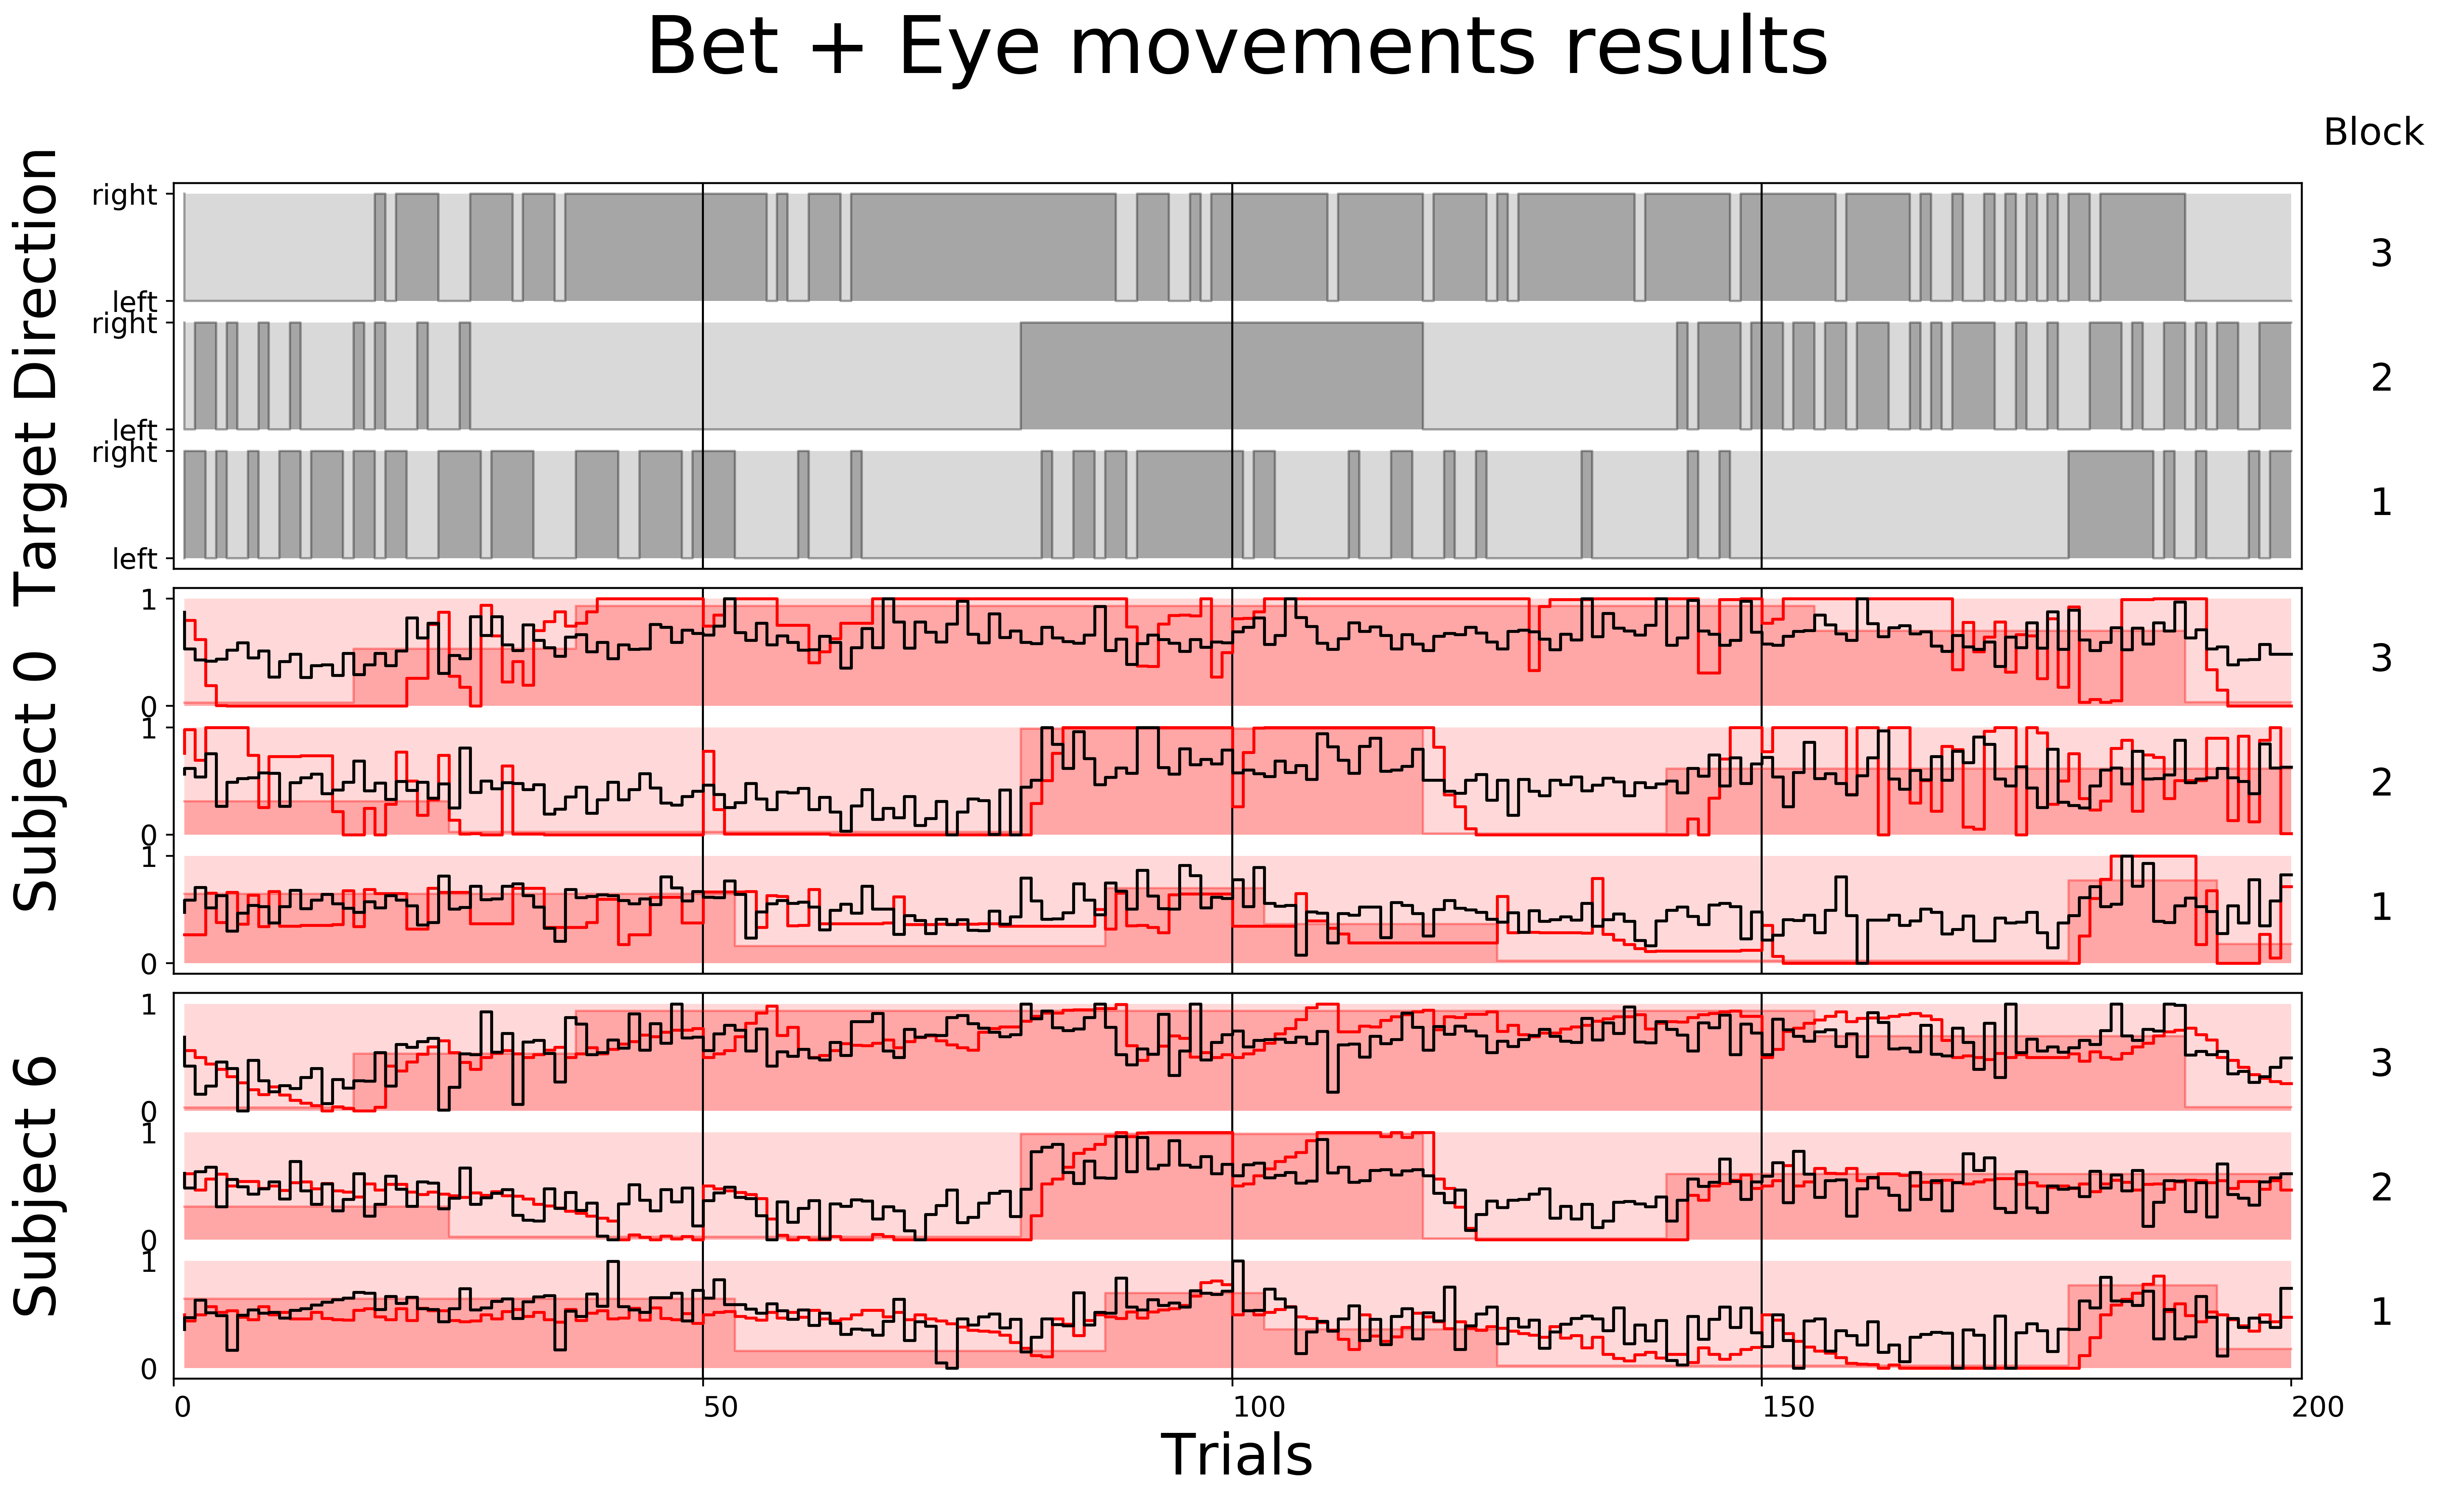
\includegraphics[width=1\linewidth]{results_enregistrement}
%\end{center}

%Let's plot the acceleration of anticipation (slope of aSPEM) as a function of the real probability at every given trial :

%\begin{center} 
%    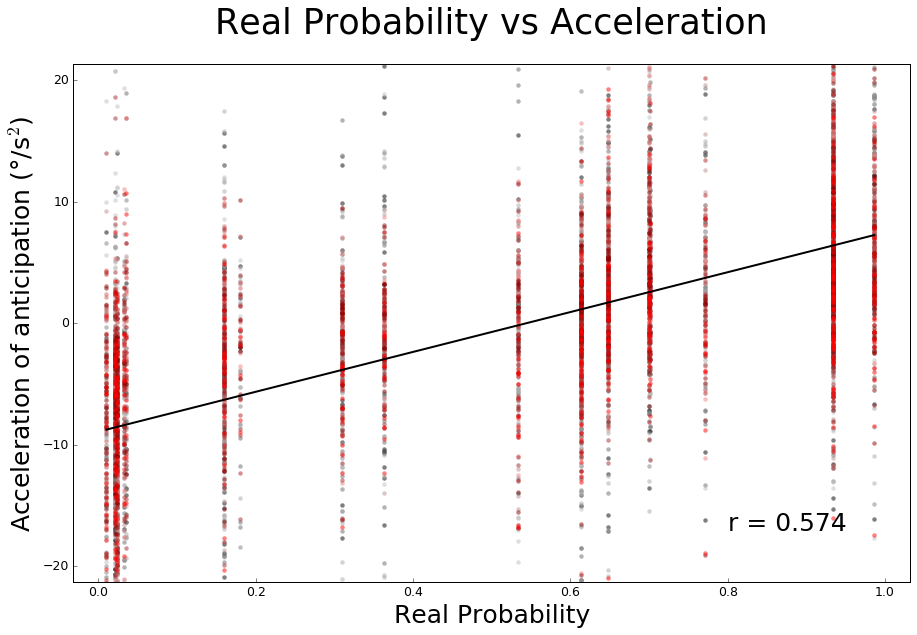
\includegraphics[width=1\linewidth]{p_real--v_a}
%\end{center}

Let's plot the value of the bet (probability bet)  and the acceleration of anticipation (slope of aSPEM) as a function of the real probability at every given trial :
%
%\begin{center} 
%    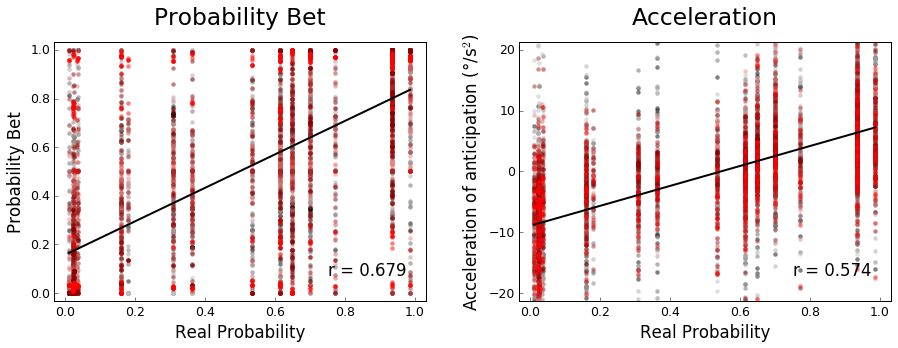
\includegraphics[width=1\linewidth]{P_real}
%\end{center}


 Let's use our model on the different sequences that were generated in our experiments in the different blocks.

we the same arrangement of panels, we show below the dynamical evolution of beliefs and above the resulting readout from the model

we see that as in the synthetic example above, there is a correct detection of switch after a short delay of a few trials

in particular, from this correct detection, the value of the inferred probability approaches the true one as the number of observations increase in one subblock.

again, we see that a fixed length model gives a similar output but with the two disadvantages described above

Let's now see how this applies to our experimental results by comparing human observers to our bayesian agent.

Which give a strong and positive Pearson coefficient.



Among our 12 subjects, we show four representative examples. we will use the same figure as in the section with raw results

but we superposed to our 2 variables, the value of the readout inferred probability along with the confidence interval.

compared to the raw results which were using the true (hidden) probability, it seems qualitatively that it follows well the traces observed experimenetally
- first, both have similar delays in ddetercting a switch, reflecting the diuffusion of probability
- second, precisions seems to increase in bigger sub-blocks as a function of the inferred run-length

as a result, the inferred probability as a function of time constitutes a useful regressor


\subsection{Relating the Bet to the Recording}

We now compare the value of bet during the bet experiment with the acceleration of anticipation during the recording :



I show here a typical velocity traces for one subject / 2 trials

- x-axis is time in milliseconds aligned on target onset, and we show respectively from left to right the fixation in gray, the GAP in pink (300ms) and the run in light gray.

- y-axis is the velocity as computed as the gradient of position. Remark that the eyelink provides with the periods of saccades or blinks that we removed from the signal. it is quite noisy and to complement existing signal processing methods, Chloe implemented a robust

- fitting method which allows to extract some key components of the velocity traces: maximum speed, latency, temporal inertia ($\tau$) and most interestingly acceleration before motion onset. We cross-validated that this method was givinfg similar results to other classical methods but in a more robust fashion/

While being sensible to recording errors, this allows us to extract the anticipatory component of SPEMs and..


 * I show here the overlay of this variable on the plot of probability biases

 * these accelarations values were here scaled according to their extremal values.

 * there seems to be a trend with the polarity of the acceleration being negative for p values below .5 and positive for values above .5

... to make this clearer, and because we used the same sequence, we can overlay the results of both experiments in one plot:

which qualitatively confirms such an intuition...

%\begin{center} 
%    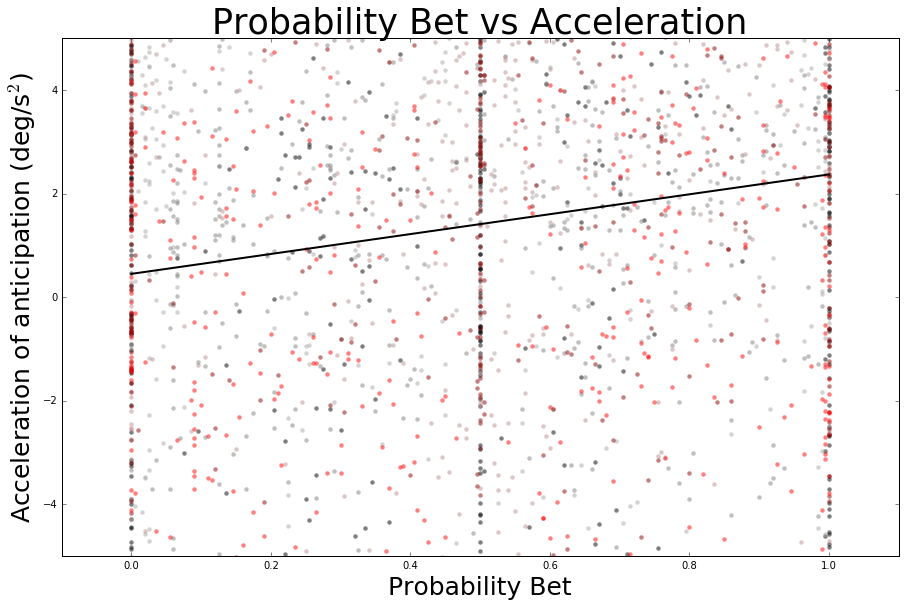
\includegraphics[width=1\linewidth]{p_parie--v_a}
%\end{center}

%\begin{center} 
%    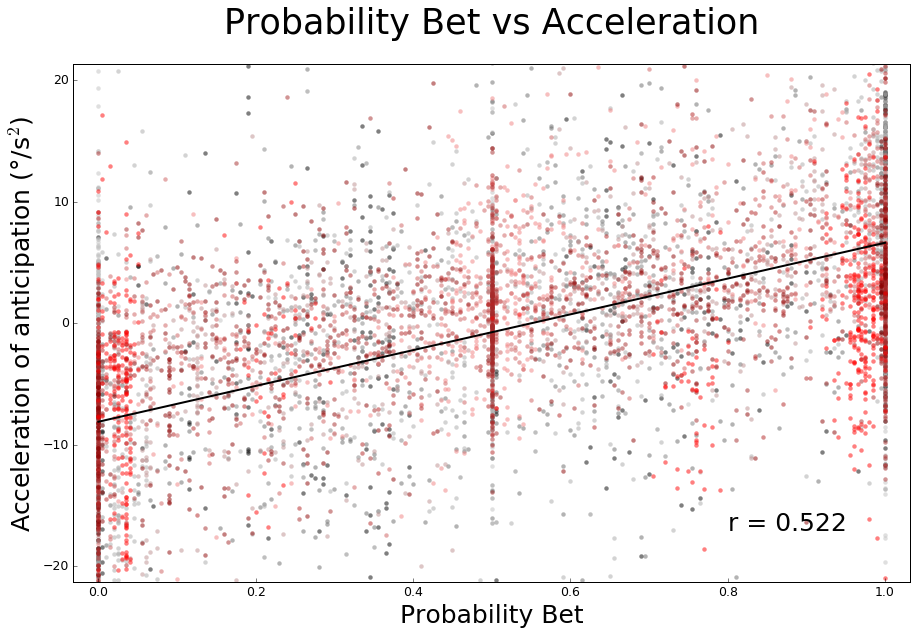
\includegraphics[width=1\linewidth]{p_bet--v_a}
%\end{center}


%\begin{figure}[H]
%\centering
%\begin{subfigure}{1\textwidth}
%\includegraphics[width=1\textwidth]{data_fit_S18.pdf}
%\phantomcaption{\label{fig:data_fit_S18.pdf}}
%\end{subfigure}
%\caption[Todo]{Fit between the probability predicted by the BCP algorithm (in red with error bars) $\hat{p}$ (for the sequences of events (rightward and leftward trials) that we used for our different experimental blocks) and the experimental datas obtained by participant 18.~\textbf{NB:} To observe the fit in an appropriate range between 0 and 1, the data for participant 18 was normalized and re-centered with the following transformation method:$\widetilde{aSPEM} = \frac{aSPEM_t-Min(aSPEM)}{Max_(aSPEM)-Min(aSPEM)}$.
%\label{fig:data_fit_S18.pdf}}
%\end{figure}

 Finally we wanted to look at the fit between aSPEM velocities and the probability $\hat{p}$ computed by the BCP algorithm at the moment of the eye movements for participants that undergo the experimental conditions of baseline, braker and booster. As we can see on fig~\ref{fig:final_reg.png}, the probability $\hat{p}$ computed by the BCP algorithm has a positive linear relationship with the aSPEM velocity. Interestingly, we can note that after computed $\hat{p}$ of around $\hat{p} > .727$, velocities in the braker condition tend to have a negative influence on the slope of the linear regression. On the booster condition we observe a higher correlation coefficient than in the baseline which is coherent with the results of study 1~(page~(\pageref{chap:4})).


 * quantitatively, one can now plot the results for all subjects

 * the x-axis corresponds to the probability that was coded at the second layer and which is unknown to the observer
 * the y -axis shows either the bet or the
 * dots represent single responses - the saturation giving the identity of the observer

 we notice a quite nice linear correlation (black line) for both experiments; of the order of that found in the classical experiment with fixed blocks and a vartiety of bias values. This is surprising as the blocks are of random length, observer can still adapt to such a volatile environment.

Another visualization, the scatter plot of acceleration  as a function of probability bet shows also that there is a correlation between both  variables.

This allows to make a first point: it is possible to use more genreal models such as hierarchical generative models.

However, while this results seem encouraging, a more finer analysis may be necessary.

\subsection{Comparing the Bayesian change point model with humans}

We now compare the individual guesses during the bet experiment and the acceleration of anticipation during the eye movement recordings with the model simulations :


%-------------------------------------------------------------%
%: FIGURE 4  fig:results_psycho
% TODO présente les résultats osycho : 1/ un sujet caractéristique 2/ 
\begin{figure}%[b!]
%\vspace{2mm}
% cf 3_Results_2.ipynb
\begin{center} 
    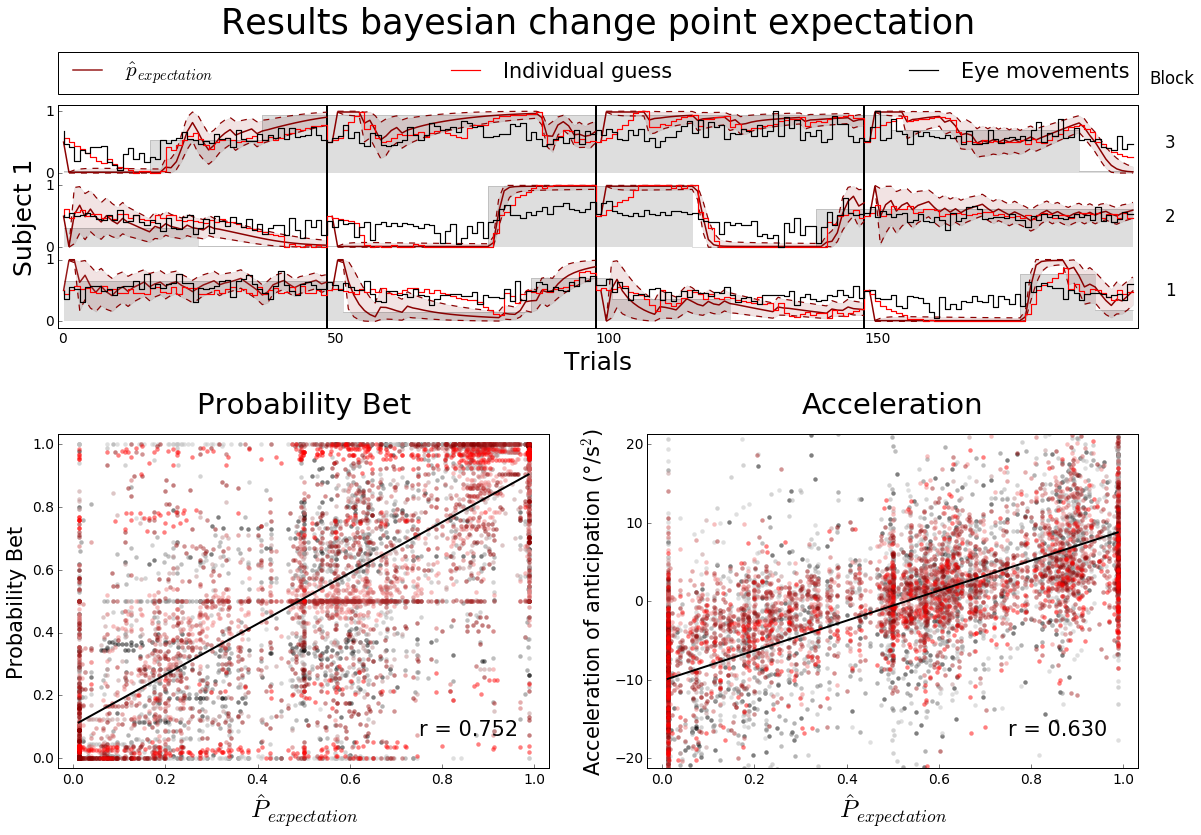
\includegraphics[width=1\linewidth]{results_bayesianchangepoint_e}
    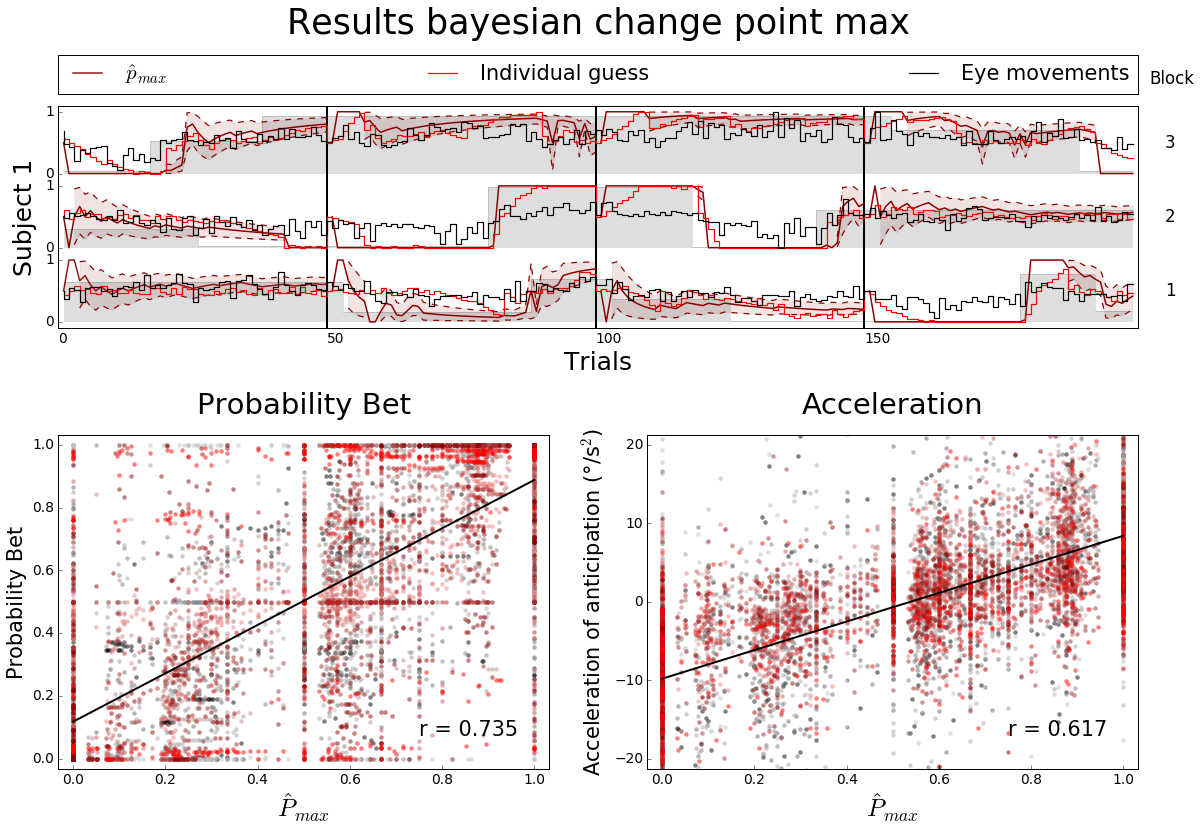
\includegraphics[width=1\linewidth]{results_bayesianchangepoint_m}
\end{center}
\caption{\emph{Psychophysical results over all participants} 
Kernel Density Estimation (KDE) of the relationship between $p$ (abscissa) and \textbf{(A)} VEM and \textbf{(B)} the value of bet (in ordinates). In \textbf{(A)}, we have overlaid is a regression line which shows a high correlation factor (R=XXX) which is superior to that found with the fixed-length design (see Appendix ...) but also with other models described in the text (fixed-length estimatyor, maximum BCP - see Appendix ... ). In \textbf{(B)}, we have fitted the data with a logistic regression showing a negligeable intercept (no bias) linked to the symmetry of the problem, but a consistent slope showing an aversion to risk (cf Kanehman).
%\textbf{(C)}  
}
\label{fig:results_psycho}
\end{figure}
%-------------------------------------------------------------%

include the comparison with a control agent, the forgetful agent with time characteristics $\tau$


we therefore used a kernel density estimation which clearly show the relationship between the agent probability and that reported by human observers
- on the right, we

to summarize, we have shown that
- there is a correlation in the anticiapatory response of eye movements in a volatile environment that is captured if we know the true probability
- that a fixed length models captures some of this correlation, but that
- our online bayesian changep[oint model better captures this correlation and that this may hint at the neural mechanisms used to anticipate in a dynamic environment

the brain is not strongly a bayesian machine, but weakly



\subsection{Analyzing inter-individual differences}

By extracting the parameters for every subject we can expect to characterise inter individual differences. 

%-------------------------------------------------------------%
%: FIGURE 5  fig:results_psycho_inter
% TODO présente une meta analyse qui montre une correlation par sujet (scatter plot) entre h_a et h_bet (see 2017-11-16 chloe figures.pdf ) y-a-til un continuum entre explorateurs et conservatezurs?, voir de montrer une causalité entre les 2 expériences - on pourrait superposer aussi les résultats si on avait utilisé un fixed-length ?
\begin{figure}%[b!]
%\begin{center} 
%    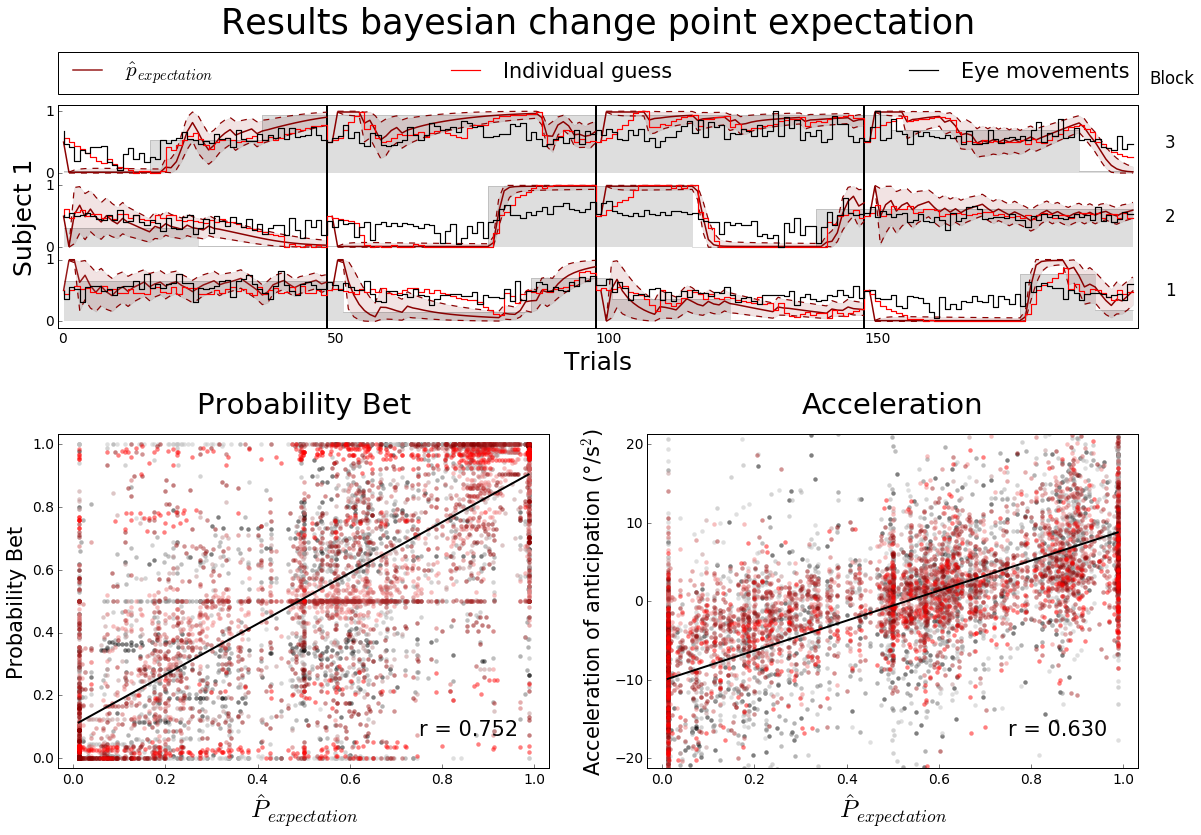
\includegraphics[width=1\linewidth]{results_bayesianchangepoint_e}
%    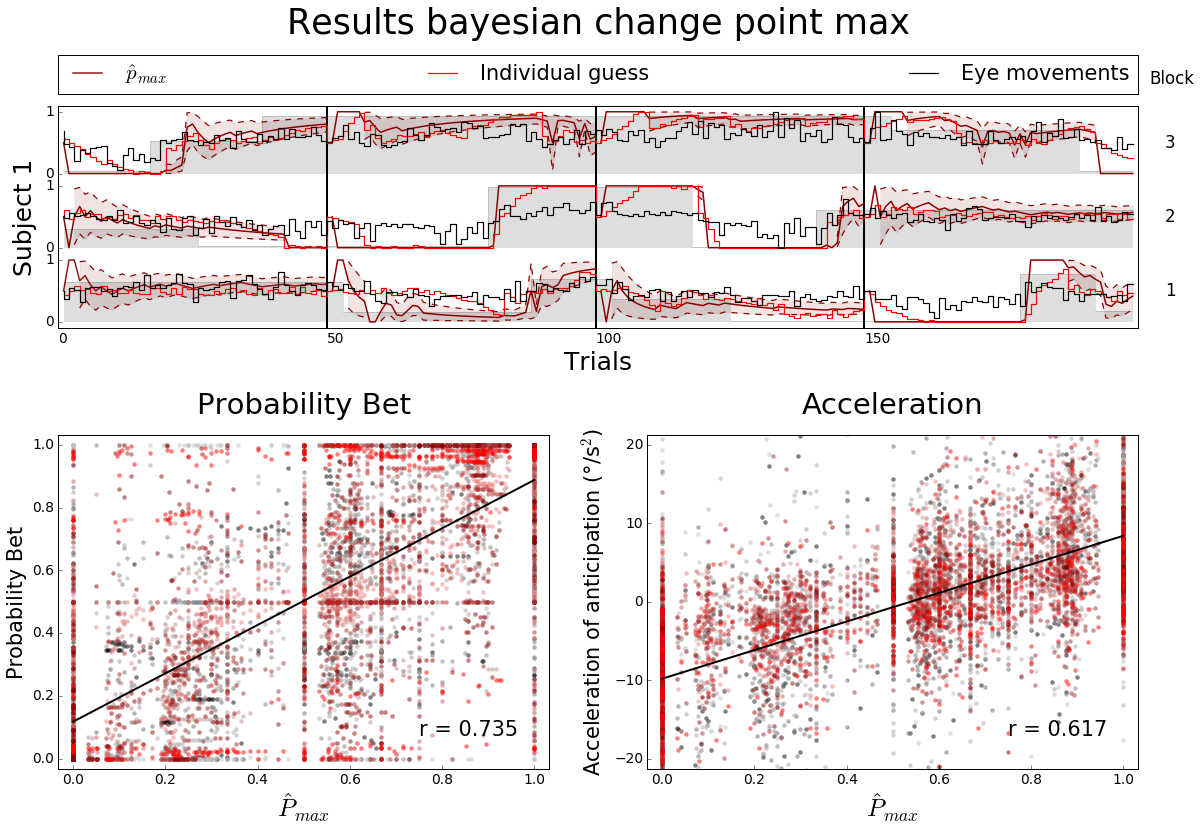
\includegraphics[width=1\linewidth]{results_bayesianchangepoint_m}
%\end{center}
\caption{\emph{Analyzing inter-individual differences} \textbf{(A)} 
\textbf{(B)} 
\textbf{(C)}  }
\label{fig:results_psycho_inter}
\end{figure}
%-------------------------------------------------------------%

There are a spectrum of individual choices between exploration and exploiting behaviors.


%: %%%%%%%%%%%%%%%%%%%%%%%%%%%%%%%%%%%%%%%%%%%%%%%%%%%%%%%%%%%%%%%

\section{Discussion}


%The oculomotor system has to constantly update its knowledge about the environment. An ordeal is then to adapt to changes with the shortest delays. Early studies have proposed that stimuli provides information to modulate reaction times within sequences~\citep{Hyman1953, Tune1964, Schvaneveldt}. This theoretical approach is coherent with the notion of local transition probabilities that quantifies at which extent an observation deviates from the preceding ones~\citep{Meyniel2016}. The way expectations act on cognitive processes has been investigated by a wide range of domains such as predictive coding~\citep{Wolpert2000, Wacongne2012}, active inference~\citep{Friston2010}, motor control~\citep{Sutton1998, Behrens2007} and reinforcement learning~\citep{Nassar2012}. Non-stationary observations can also explain why both local and global effects emerge and why local effects persist in the long run even within purely random sequences~\citep{Cho2002, Yu2009}. This constant update of a general belief on the world can be a consequence of the constant attempt to learn the non-stationary structure of the environment that can change at unpredictable times~\citep{Yu2009}. Many studies have actually already pointed the brain's ability to apprehend non-stationary states in environments~\citep{Ossmy2013, Meyniel2015}. As explained by~\citet{Meyniel2016}, the belief upon an environment can be divided in two different ways:
%
%\begin{enumerate}[label=\Alph*)]
%\item Update the~\textit{a priori} likelihood of a sudden change, also known as the volatility and taken into account by the model~\citep{Behrens2007} 
%\item A leaky integrator factor imbedded in the model~\citep{Anderson2006, Yu2009, Ossmy2013, Wang2002}
%\end{enumerate}
%

%: theory / computationnally-driven experiments 
% it's a main novelty
genrative models for changing environments allows to know the ground truth compared to natural stimulation (see Rust eand Movshon)%
Let's remember our hierarchical generative model.

At any given trial, we wish to construct an algorithm which

We will introduce a fundamental component of Bayesian models : a latent variable

this new variable will be used to test different hypothesis which will be evaluated to predict future states. it is called latent because it aims at representing a variable that is latent (or hidden) to the observer

in our case, we will assume that the bayesian model knows about the structure of the generative model and we will set it to the current run-length $r$, that is, at any given trial, the hypothesis that the past r observations belong to the same block. of course a wrong choice of a latent variables (let's say the temperture in the experimental room) may give unexpected results, even is the bayesian model is "optimal" - an essential point to understand in bayesian inference

extension to multi-nomioal( daniele + fred danion)



% Still, only Bayesian models recover an explicit probabilistic representation of change in likelihood. Recent experimental studies suggest, indeed, that the brain is able of estimating a hierarchical model of the environment and that humans can explicitly report sudden changes in sequences~\citep{Meyniel2015, Gallistel2014}. Ultimately, we passed over one of leaky integrator models' main default, having a too fixed and rigid memory parameter. In our work the memory parameter is constantly inferred by the BCP algorithm over the observation of the number of trials where this inference stayed reliable and then globally represented probabilistic representation of changes in likelihood and actualization of~\textit{a priori} knowledge.


perspectives:
- RL : use hindsight example of localization for saccades: get the changepoints then improve estimate of reward allows to optimize the association between the set of measures and their utility (compared to Q-learning where it is a fixed length)
- interindividual differences : markers for the berhaviour traces - traces of the network implementation
- the brain is weakly Bayesian (it does not care about equations but more about sugar)


%: %%%%%%%%%%%%%%%%%%%%%%%%%%%%%%%%%%%%%%%%%%%%%%%%%%%%%%%%%%%%%%%

\section{Conclusions}


\begin{itemize}\setlength{\itemsep}{0ex}
\item There is a strong correlation between the real probability and the value of the bet,

\item there is a stong correlation between the strength of anticipation and the probability of the process,

\item we have developed a Bayesian model of an agent estimating the probability of changing points. This allows to dynamically infer the direction probability and directly compare model and human behaviour.

\end{itemize}

{\tiny
\printbibliography
}
%%%%%%%%%%%%%%%%%%%%%%%%%%%%%%%%
\end{document}%
